% !TEX root = thesis.tex
% !TEX encoding = Shift_JIS
% !TEX spellcheck = none
%
% 2016.06.16 初版
% 2019.01.04
% 2020.12.22
%
% thesis.tex
%
%
%
%
\documentclass[12pt,titlepage]{jsarticle}
%
\usepackage[dvipdfmx,draft]{graphicx}	% 自分で加えた	by 野田
%
\usepackage{amsmath}			% 自分で加えた	by 野田
\usepackage{url}					% 自分で加えた	by 野田
\usepackage{comment}			% 自分で加えた	by 野田
\usepackage{supertabular}		% 自分で加えた	by 野田
\usepackage{cite}					% 自分で加えた	by 野田
\usepackage{here}				% 自分で加えた	by 野田

%\usepackage[footskip=11truemm,top=15truemm,bottom=20truemm,left=20truemm,right=15truemm]{geometry} %ページの余白を調整したいときは,ここの数字を触る.実寸のミリメートル

%●nag Detecting and warn?ing about obsolete LaTeX commands
%  http://www.ctan.org/tex-archive/macros/latex/contrib/nag
%  LaTeX文書の冒頭に
%\RequirePackage[l2tabu, orthodox]{nag}
%  と書いておくと古いコマンドやパッケージの利用を警告してくれます.
%
%●onlyamsmath  Inhibit use of non-amsmath mathe?matics markup when using amsmath
%  http://www.ctan.org/tex-archive/macros/latex/contrib/onlyamsmath
%\usepackage[all, warning]{onlyamsmath}
% で amsmath が提供しない数式環境を使用した場合に警告してくれます.



\title{\vspace{-15mm}{\LARGE 2022年度 卒業論文}\\\vspace{25mm}
\huge 製造業向けロボットを知能化する\\自律システムアルゴリズムの研究\vspace{20mm}\\}
%

\author{ 
\Large 大阪工業大学 ロボティクス&デザイン工学部\\\\
\vspace{5mm}\Large ロボット工学科\\
\vspace{5mm}\Large %産業用ロボット研究室
\vspace{0mm}\\
{\huge 工大 ロボ太郎} \vspace{14.5mm}\\
\\\Large 指導教員\\\\\vspace{-4.0mm}
\vspace{0mm}\Large 野田 哲男 %印
}

%
\date{}

%
\begin{document}

\maketitle
\newpage
%
% 内容梗概
%
\thispagestyle{empty}
\section*{内容梗概}
% !TEX root = thesis.tex
% !TEX encoding = Shift_JIS
% !TEX spellcheck = none


製造業分野では少品種大量の製品を高品質にライン生産してきたが,2000年代に入って多様化する市場ニーズに応えるため,人の知能をより積極的に援用する人セル生産方式を導入した.しかし人セル生産方式の生産能力はライン方式に比して低位で,作業者スキル由来の品質ばらつきは直近の課題であり,中長期的には生産人口減少問題と無縁ではない.そこで本研究では,ライン方式と人セル方式のそれぞれのメリットを集めたセル生産ロボット方式を実現するためのロボット知能化技術に取り組んだ.そのなかで知能としてとりわけ自律性が重要なことがわかった.よって本論文では製造業向けロボットに自律性を付与するシステムアルゴリズムを開発し,以下の結果を得たことを論述する.

まず,人の自律性を特徴づける試行錯誤による習熟を,未知の目的関数の最適化問題と定式化して解く独自の「能動型探索アルゴリズム」を提案する.これは,その問題設定と,その試行で得られるであろう情報量・情報が得られないリスク量を同時に考慮して次の試行を最適化する点とに独創性がある.実証実験の結果,熟練者の調整で動作時間1045.33[ms]のロボット軌道が,約56\%の590.22[ms]に短縮したこと,さらに熟練者による加工機制御パラメータ調整などの同種の困難性を持つ問題への水平展開に成功したことで,有用性が示される.

次に,組立工程で切望されるバラ積み状態の部品供給に取り組む.これはロボット学にとってランダム・ビン・ピッキングという未解決の古典的難題である.この問題を複数の小問題に分割して解くシステム解法と,作業計画の試行錯誤を実行する「持ち替えグラフアルゴリズム」とを提案する.これらは既に有りそうで実は無かった方法である点,実行可能解を網羅的に算出する点に独創性がある.実証システムにおいて,数[g]から数10[g]の質量の実際の小型電機製品を構成する11種類以上の金属およびプラスチックの部品を,最速2秒台後半の時間間隔にて指定された姿勢に整列させられ,新規部品の追加に要するエンジニアリング時間は部品一つ当たり0.5日であることから,有用性がある.

\endinput


%
% 目次
%
\newpage
\pagenumbering{roman} % NODA added
\setcounter{page}{1}    % NODA added
\tableofcontents
\newpage
\listoffigures
\listoftables
\newpage
%
\pagenumbering{arabic} % NODA added
\setcounter{page}{1}    % NODA added

%
%
% 本文
%
%

% for DEBUG % 
% !TEX root = thesis.tex
% !TEX encoding = Shift_JIS
% !TEX spellcheck = none


\section{序論}
\subsection{はじめに}

本論文の主題は,第4章と第5章に示す自律システムアルゴリズムである.
同アルゴリズムの研究開発に辿り着くまでには,各時代の要請の変遷とそれを解決するための研究開発の経緯があった.
そこで,なぜ3章以降の開発が必要になったかを明確に定義づけるため,
解説論文的な記述にはなるが,本章と第2章でこれらを示すことにする.

第3章ではそれらを踏まえて開始した,自律型セル生産ロボットシステム技術プラットフォームの
開発プロジェクトの概要について述べる.これはオープンイノベーションを活用した数十人規模の
一大プロジェクトであった.

第4章および第5章で,同プラットフォームに対する要求のなかで最も困難性の高い課題を解決するための
自律システムアルゴリズムについて報告する.




\subsection{背景と動機}

生産人口の減少は,まず日本が,その後,世界が必ず直面する構造問題である.これに対し,あらゆる分野に自動化を万遍なく普及させることが,安全安心で豊かな未来を維持発展させる方法の一つとなる.

製造業分野に目を向けると,動力を利用するようなった産業革命以来,生産を自動化して安価で高品質な製品を大量にライン生産することで,豊かな生活の実現に貢献してきた.
ライン生産方式というソリューションは,設備投資コスト・運用コストを長い期間をかけて回収することが前提であり,つまり概してそれらのコストは大きくなるデメリットがあるものの,一度構築して安定して運用できるようになれば,高速で安定した生産の自動化を維持することにより,同じ品質の製品を大量に製造することができることがメリットとなる.ライン生産方式に投入されるロボットは,この目的のためにその機能を最適設計され,製造されている.そのようなロボットの行動計画は,ライン構築技術者がライン構築時に知恵を絞って設計し,生産活動開始後は,ロボットはあらかじめ定められた単純な位置決め動作を高速に繰り返すことのみに特化していた.これは,動物が条件反射で運動していることに相当する.1990年代にはいると,二次元ビジョンセンサが普及しはじめ,多少の位置ずれをロボット自ら修正する意味での知能化が実用化したが,やはり単純な位置決め動作を高速に繰り返すことに主眼が置かれていて生産ラインの一部への導入にとどまっていた.

2000年代に入ると市場ニーズが多様化しはじめ,短期間のうちに生産機種を切り替える必要が生じた.
このような状況の変化に低コストで柔軟に実施できる人セル生産方式と呼ばれるソリューションが新たな選択肢として注目され,同方式をフル活用したEMS(
\underline{E}lectronics
\underline{M}anufacturing
\underline{S}ervice)事業者も躍進した.
しかし,セル生産方式の生産能力はライン方式に比して低位である.さらには作業者の熟練度に依存する品質のばらつきが直近の課題として取り沙汰されるようになり,これらを解決するために労働者の選抜制をとるなどの方法が取られた.さらには景気の変動に応じて雇用を増減することなどもあわせて,これらの非人道な対応が社会問題となった.また,このような人手をあてにした方式は中長期的には生産人口減少の影響と無縁ではない.

やがて2000年代後半になると,冒頭で述べた生産人口減少問題がようやく人口に膾炙するようになり,
実際に統計的にも日本の人口が減少しはじめ,少子高齢化,生産人口の減少が現実のものとして議論されるようになった.同時に新興国の工業化と市場化の進展により国際競争が激化し,半導体製品・電気電子製品の設計製造技術の革新,景気変動・為替レートの変容・市場ニーズの激変に対応するための市場オフショア生産と地産地消と生産拠点国内回帰の選択の混乱,および市場のグローバル化といった複雑な事象が急速に同時進行したことで,次世代のものつくりの方式が求められ始めていたのが,この2000年代後半の展開であった.

著者らの研究グループでは複雑な状況に対応するためのソリューションの選択肢を増やすため,2006年に新規の研究プロジェクトをスタートさせ,ライン方式,人セル方式,それぞれのメリットを集めたセル生産ロボット方式の実用化を目指すことにした.
ライン生産方式は上述のごとく品種の生産期間は長いことを前提とし少品種大量生産のために最適化され,生産される品質も安定している.ライン生産のなかで産業ロボットは,ワークや治具をピック・アンド・プレースする単純作業に投入されていた.一方,人セル生産方式は生産品種の切り替えが数か月未満で行われることを前提とし,生産速度よりも機種切り替えコストを重視した最適化の結果となっていた.生産速度はラインに比して低いがセルを並列化することで補うという考え方であった.品質は人に依存してばらつきが大きくなっていた.

これに対し,本研究で提案するセル生産ロボット方式では,品種切り替えは迅速,生産速度はそこそこだが品質は安定しているという良いところ取りを目指し,生産速度の増減は,セルの並列数を変化させることで対応しようという概念となる.
ここまで述べてきたことを概念的に図\ref{fig:ChangesInManufacturing}にまとめる.

\begin{figure}[b]\centering 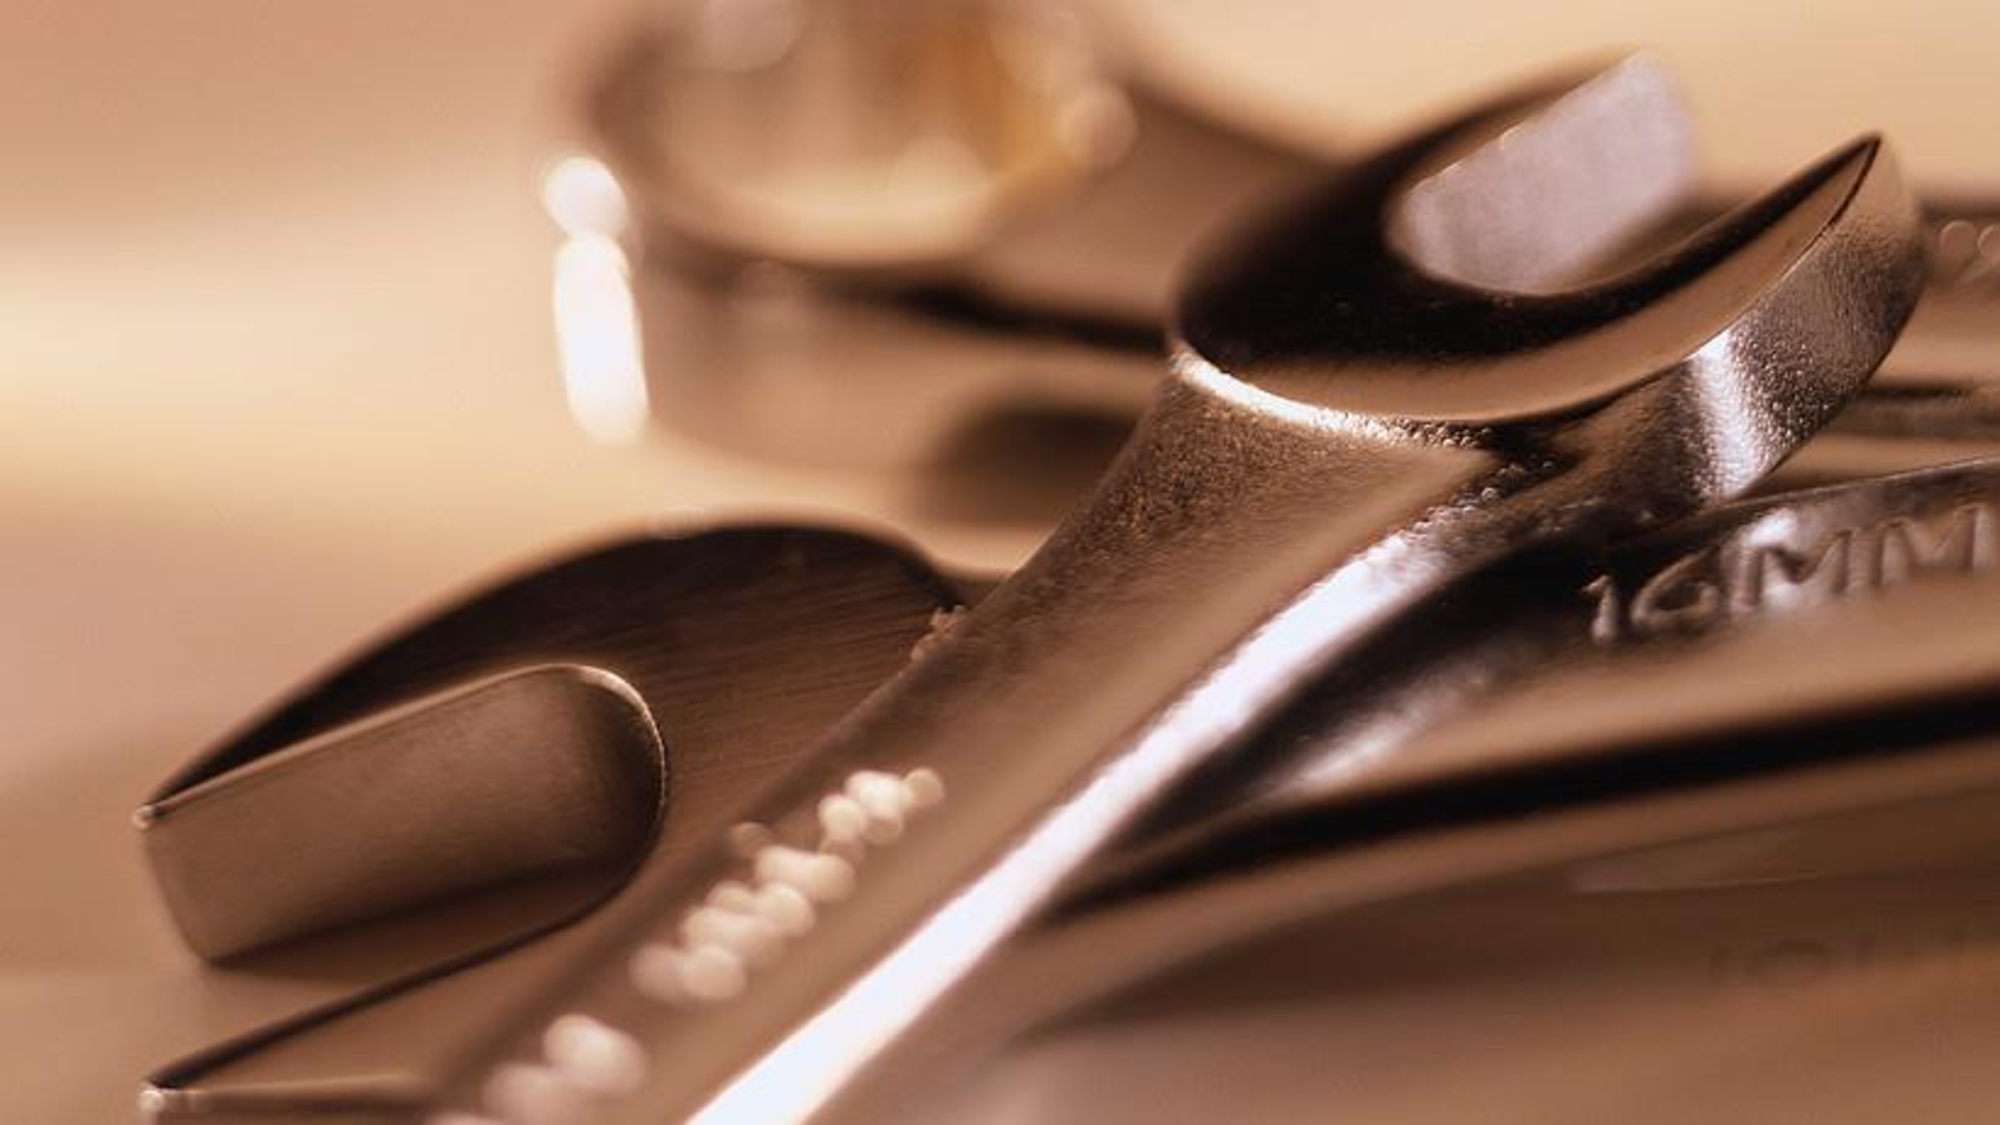
\includegraphics[width=12cm]{Fig/ChangesInManufacturing.pdf}
\caption{製造業におけるニーズとソリューション選択肢の変遷}\label{fig:ChangesInManufacturing}\end{figure}


\subsection{問題の本質の同定}

もともとロボット単体で生産セルを構成するという基本的な考え方は,すでに1980年代の後半に提案されている\cite{Zupancic1988}.当時,人工知能研究もエキスパートシステムと呼ばれる実用化が見られるようになり,バックプロパゲーション則の発見によるニューラルネットワークや,直接法Fuzzy推論則によるFuzzy制御の応用,遺伝的アルゴリズムの応用などが進展しはじめた時代背景とあいまって,生産分野でも,工作機械など熟練者の手に委ねられてきた生産財の知能化研究と実用化が進められてきた.

しかしながら,それらの研究開発成果は,自動化には成功するものの,この手の知的制御システムを
構築するにあたり,熟練作業者モデルを構築するためのシステムの開発,および熟練作業者モデリングの困難さは課題として残ることになった.さらには,1990年代後半から2000年にかけて生産システムの規模が年々大きく複雑化しはじめ,システム構築が属人的技能にとどまっている点も大きな問題となり始めていた\cite{Noda2004}.
2000年代後半になると,産業現場の実務上の問題として,エンジニアリングコストの大きさがシステム構築のボトルネックとなっていることが,はっきりと認識されるようになった.エンジニアリングは,属人的な知識集約作業の典型例であり,リードタイムの長さもコストの一部として計上される.

そこで,著者らの研究グループではこのエンジニアリングコストの削減のため,問題の分析を実施し,本質的な解決策として必要な知能化機能を同定した.これを,第2章で詳報する.

通常,ロボットの知能化というと,外界センサーフードバックにより従来できなかった複雑な動作軌道を実現することに主眼が置かれるが,著者らの研究グループの独創性は,現場のニーズに直接立脚した点にある.
産業用ロボットは生産財である.このため,知能を持った新しいロボットが安全・高速・安定な繰り返し作業を,従来方式となんら変わりなく実現することは大前提である.そのもとで,生産品目切り替えや誤った部品の混入などの大きな外乱に柔軟に対応すること,繰り返し作業への習熟といった自律性を発現する必要がある.
つまり複雑な作業が可能となったとしても動作速度が落ちてしまったり,投資コストが大きくなってしまったりすると,現場では受け入れられない.従来型の生産システムが採用され,極端な場合は作業者を雇い入れるといった解決策が取られることになる.

また,エンジニアリングコストの削減に注目することは,これまでにない視点であり独創性が高い.\cite{robotneeds}%参考文献引用例


\begin{table}[tb]
  \centering
    \caption{値段表}
  \begin{tabular}{|l|c|r||r|} \hline
    メニュー & サイズ & 値段 & カロリー \\ \hline \hline
    牛丼 & 並盛 & 500円 & 600 kcal \\
    牛丼 & 大盛 & 1,000円 & 800 kcal \\
    牛丼 & 特盛 & 1,500円 & 1,000 kcal \\ \hline
  \end{tabular}
\end{table}


\subsection{研究開発のグランドデザインと本論文の主題}

このもとで,知能化技術の要素を開発し,技術プラットフォームとして統合することにした.このことを第3章で詳報する.
そこでは,それぞれの課題の解決のための知能化技術の開発を進めていることを述べる.

研究開発を進めるなかで,人の知能のうち,とりわけ自律性が重要な役割を担っていることがわかったので,製造業向けロボットに自律性を付与する各システムアルゴリズムを開発することにし,これを本論文の主題とした.

まず,人の自律性の最たる特徴の試行錯誤による習熟を,未知の目的関数の最適化問題として定式化して独自の自律システムアルゴリズム「能動型探索アルゴリズム」を提案し,実際のシステムで効果を確認した.また,同種の困難性を持つ問題に対し効果を確認した.これは第4章で詳報する.

次に,自動化システムにおける製品組立作業ではバラ積み状態の部品供給が必ず問題となる.そこで多品種部品のバラ積み供給を実現するシステム設計理論と動作の試行錯誤を実行する「持ち替えグラフアルゴリズム」を提案し,実際の現場で効果を確認した.これは第5章で詳報する.\newpage



\subsection{本論文の構成について}
\noindent
次章以降を,上述した内容に沿って,以下の6つの章で構成する.\\

\noindent
第2章では,自動化システム研究の現状を分析し,課題を明らかにする.\\

\noindent
第3章では,課題を解決するための技術プラットフォーム「自律型セル生産ロボットシステム」の全容について述べる.\\

\noindent
第4章では,課題として重要な自律性の発現について,動作習熟のための自律システムアルゴリズム「能動探索アルゴリズム」について述べる.\\

\noindent
第5章では,おなじく自律性の発現について,バラ積み部品供給のための自律システムアルゴリズム「持ち替えグラフ」について述べる.\\

\noindent
第6章では,実際の製品組立作業を実行するセル生産ロボットシステムを構築して開発技術を検証した結果を報告する.\\

\noindent
第7章で,全体を通じての結論を述べる.\\



\endinput

% for DEBUG % 


% for DEBUG % \setcounter{chapter}{1}
% for DEBUG % 
% !TEX root = thesis.tex
% !TEX encoding = Shift_JIS
% !TEX spellcheck = none


\section{序論}
\subsection{はじめに}

本論文の主題は,第4章と第5章に示す自律システムアルゴリズムである.
同アルゴリズムの研究開発に辿り着くまでには,各時代の要請の変遷とそれを解決するための研究開発の経緯があった.
そこで,なぜ3章以降の開発が必要になったかを明確に定義づけるため,
解説論文的な記述にはなるが,本章と第2章でこれらを示すことにする.

第3章ではそれらを踏まえて開始した,自律型セル生産ロボットシステム技術プラットフォームの
開発プロジェクトの概要について述べる.これはオープンイノベーションを活用した数十人規模の
一大プロジェクトであった.

第4章および第5章で,同プラットフォームに対する要求のなかで最も困難性の高い課題を解決するための
自律システムアルゴリズムについて報告する.




\subsection{背景と動機}

生産人口の減少は,まず日本が,その後,世界が必ず直面する構造問題である.これに対し,あらゆる分野に自動化を万遍なく普及させることが,安全安心で豊かな未来を維持発展させる方法の一つとなる.

製造業分野に目を向けると,動力を利用するようなった産業革命以来,生産を自動化して安価で高品質な製品を大量にライン生産することで,豊かな生活の実現に貢献してきた.
ライン生産方式というソリューションは,設備投資コスト・運用コストを長い期間をかけて回収することが前提であり,つまり概してそれらのコストは大きくなるデメリットがあるものの,一度構築して安定して運用できるようになれば,高速で安定した生産の自動化を維持することにより,同じ品質の製品を大量に製造することができることがメリットとなる.ライン生産方式に投入されるロボットは,この目的のためにその機能を最適設計され,製造されている.そのようなロボットの行動計画は,ライン構築技術者がライン構築時に知恵を絞って設計し,生産活動開始後は,ロボットはあらかじめ定められた単純な位置決め動作を高速に繰り返すことのみに特化していた.これは,動物が条件反射で運動していることに相当する.1990年代にはいると,二次元ビジョンセンサが普及しはじめ,多少の位置ずれをロボット自ら修正する意味での知能化が実用化したが,やはり単純な位置決め動作を高速に繰り返すことに主眼が置かれていて生産ラインの一部への導入にとどまっていた.

2000年代に入ると市場ニーズが多様化しはじめ,短期間のうちに生産機種を切り替える必要が生じた.
このような状況の変化に低コストで柔軟に実施できる人セル生産方式と呼ばれるソリューションが新たな選択肢として注目され,同方式をフル活用したEMS(
\underline{E}lectronics
\underline{M}anufacturing
\underline{S}ervice)事業者も躍進した.
しかし,セル生産方式の生産能力はライン方式に比して低位である.さらには作業者の熟練度に依存する品質のばらつきが直近の課題として取り沙汰されるようになり,これらを解決するために労働者の選抜制をとるなどの方法が取られた.さらには景気の変動に応じて雇用を増減することなどもあわせて,これらの非人道な対応が社会問題となった.また,このような人手をあてにした方式は中長期的には生産人口減少の影響と無縁ではない.

やがて2000年代後半になると,冒頭で述べた生産人口減少問題がようやく人口に膾炙するようになり,
実際に統計的にも日本の人口が減少しはじめ,少子高齢化,生産人口の減少が現実のものとして議論されるようになった.同時に新興国の工業化と市場化の進展により国際競争が激化し,半導体製品・電気電子製品の設計製造技術の革新,景気変動・為替レートの変容・市場ニーズの激変に対応するための市場オフショア生産と地産地消と生産拠点国内回帰の選択の混乱,および市場のグローバル化といった複雑な事象が急速に同時進行したことで,次世代のものつくりの方式が求められ始めていたのが,この2000年代後半の展開であった.

著者らの研究グループでは複雑な状況に対応するためのソリューションの選択肢を増やすため,2006年に新規の研究プロジェクトをスタートさせ,ライン方式,人セル方式,それぞれのメリットを集めたセル生産ロボット方式の実用化を目指すことにした.
ライン生産方式は上述のごとく品種の生産期間は長いことを前提とし少品種大量生産のために最適化され,生産される品質も安定している.ライン生産のなかで産業ロボットは,ワークや治具をピック・アンド・プレースする単純作業に投入されていた.一方,人セル生産方式は生産品種の切り替えが数か月未満で行われることを前提とし,生産速度よりも機種切り替えコストを重視した最適化の結果となっていた.生産速度はラインに比して低いがセルを並列化することで補うという考え方であった.品質は人に依存してばらつきが大きくなっていた.

これに対し,本研究で提案するセル生産ロボット方式では,品種切り替えは迅速,生産速度はそこそこだが品質は安定しているという良いところ取りを目指し,生産速度の増減は,セルの並列数を変化させることで対応しようという概念となる.
ここまで述べてきたことを概念的に図\ref{fig:ChangesInManufacturing}にまとめる.

\begin{figure}[b]\centering 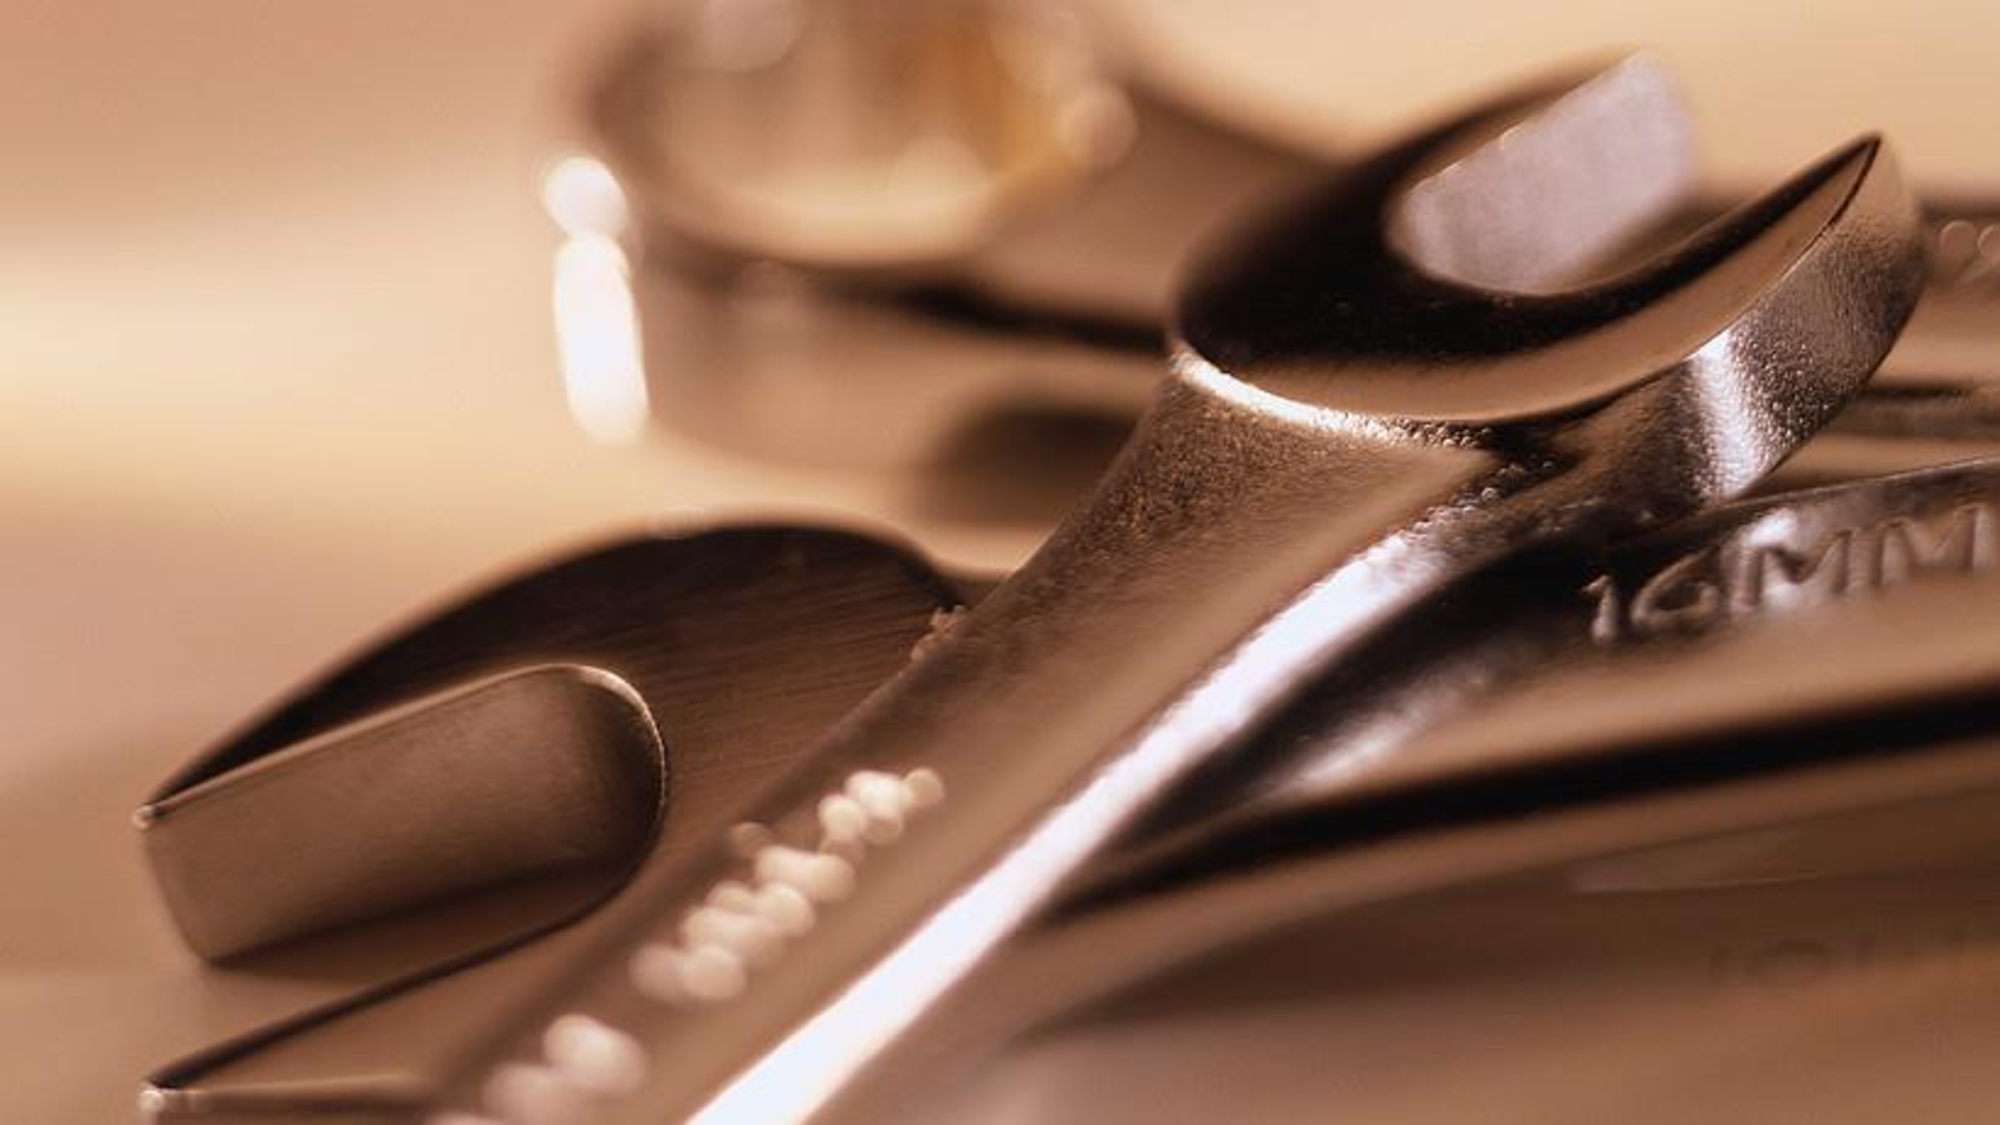
\includegraphics[width=12cm]{Fig/ChangesInManufacturing.pdf}
\caption{製造業におけるニーズとソリューション選択肢の変遷}\label{fig:ChangesInManufacturing}\end{figure}


\subsection{問題の本質の同定}

もともとロボット単体で生産セルを構成するという基本的な考え方は,すでに1980年代の後半に提案されている\cite{Zupancic1988}.当時,人工知能研究もエキスパートシステムと呼ばれる実用化が見られるようになり,バックプロパゲーション則の発見によるニューラルネットワークや,直接法Fuzzy推論則によるFuzzy制御の応用,遺伝的アルゴリズムの応用などが進展しはじめた時代背景とあいまって,生産分野でも,工作機械など熟練者の手に委ねられてきた生産財の知能化研究と実用化が進められてきた.

しかしながら,それらの研究開発成果は,自動化には成功するものの,この手の知的制御システムを
構築するにあたり,熟練作業者モデルを構築するためのシステムの開発,および熟練作業者モデリングの困難さは課題として残ることになった.さらには,1990年代後半から2000年にかけて生産システムの規模が年々大きく複雑化しはじめ,システム構築が属人的技能にとどまっている点も大きな問題となり始めていた\cite{Noda2004}.
2000年代後半になると,産業現場の実務上の問題として,エンジニアリングコストの大きさがシステム構築のボトルネックとなっていることが,はっきりと認識されるようになった.エンジニアリングは,属人的な知識集約作業の典型例であり,リードタイムの長さもコストの一部として計上される.

そこで,著者らの研究グループではこのエンジニアリングコストの削減のため,問題の分析を実施し,本質的な解決策として必要な知能化機能を同定した.これを,第2章で詳報する.

通常,ロボットの知能化というと,外界センサーフードバックにより従来できなかった複雑な動作軌道を実現することに主眼が置かれるが,著者らの研究グループの独創性は,現場のニーズに直接立脚した点にある.
産業用ロボットは生産財である.このため,知能を持った新しいロボットが安全・高速・安定な繰り返し作業を,従来方式となんら変わりなく実現することは大前提である.そのもとで,生産品目切り替えや誤った部品の混入などの大きな外乱に柔軟に対応すること,繰り返し作業への習熟といった自律性を発現する必要がある.
つまり複雑な作業が可能となったとしても動作速度が落ちてしまったり,投資コストが大きくなってしまったりすると,現場では受け入れられない.従来型の生産システムが採用され,極端な場合は作業者を雇い入れるといった解決策が取られることになる.

また,エンジニアリングコストの削減に注目することは,これまでにない視点であり独創性が高い.\cite{robotneeds}%参考文献引用例


\begin{table}[tb]
  \centering
    \caption{値段表}
  \begin{tabular}{|l|c|r||r|} \hline
    メニュー & サイズ & 値段 & カロリー \\ \hline \hline
    牛丼 & 並盛 & 500円 & 600 kcal \\
    牛丼 & 大盛 & 1,000円 & 800 kcal \\
    牛丼 & 特盛 & 1,500円 & 1,000 kcal \\ \hline
  \end{tabular}
\end{table}


\subsection{研究開発のグランドデザインと本論文の主題}

このもとで,知能化技術の要素を開発し,技術プラットフォームとして統合することにした.このことを第3章で詳報する.
そこでは,それぞれの課題の解決のための知能化技術の開発を進めていることを述べる.

研究開発を進めるなかで,人の知能のうち,とりわけ自律性が重要な役割を担っていることがわかったので,製造業向けロボットに自律性を付与する各システムアルゴリズムを開発することにし,これを本論文の主題とした.

まず,人の自律性の最たる特徴の試行錯誤による習熟を,未知の目的関数の最適化問題として定式化して独自の自律システムアルゴリズム「能動型探索アルゴリズム」を提案し,実際のシステムで効果を確認した.また,同種の困難性を持つ問題に対し効果を確認した.これは第4章で詳報する.

次に,自動化システムにおける製品組立作業ではバラ積み状態の部品供給が必ず問題となる.そこで多品種部品のバラ積み供給を実現するシステム設計理論と動作の試行錯誤を実行する「持ち替えグラフアルゴリズム」を提案し,実際の現場で効果を確認した.これは第5章で詳報する.\newpage



\subsection{本論文の構成について}
\noindent
次章以降を,上述した内容に沿って,以下の6つの章で構成する.\\

\noindent
第2章では,自動化システム研究の現状を分析し,課題を明らかにする.\\

\noindent
第3章では,課題を解決するための技術プラットフォーム「自律型セル生産ロボットシステム」の全容について述べる.\\

\noindent
第4章では,課題として重要な自律性の発現について,動作習熟のための自律システムアルゴリズム「能動探索アルゴリズム」について述べる.\\

\noindent
第5章では,おなじく自律性の発現について,バラ積み部品供給のための自律システムアルゴリズム「持ち替えグラフ」について述べる.\\

\noindent
第6章では,実際の製品組立作業を実行するセル生産ロボットシステムを構築して開発技術を検証した結果を報告する.\\

\noindent
第7章で,全体を通じての結論を述べる.\\



\endinput

% for DEBUG % 


% for DEBUG % \setcounter{chapter}{2}  
% for DEBUG % 
% !TEX root = thesis.tex
% !TEX encoding = Shift_JIS
% !TEX spellcheck = none


\section{序論}
\subsection{はじめに}

本論文の主題は,第4章と第5章に示す自律システムアルゴリズムである.
同アルゴリズムの研究開発に辿り着くまでには,各時代の要請の変遷とそれを解決するための研究開発の経緯があった.
そこで,なぜ3章以降の開発が必要になったかを明確に定義づけるため,
解説論文的な記述にはなるが,本章と第2章でこれらを示すことにする.

第3章ではそれらを踏まえて開始した,自律型セル生産ロボットシステム技術プラットフォームの
開発プロジェクトの概要について述べる.これはオープンイノベーションを活用した数十人規模の
一大プロジェクトであった.

第4章および第5章で,同プラットフォームに対する要求のなかで最も困難性の高い課題を解決するための
自律システムアルゴリズムについて報告する.




\subsection{背景と動機}

生産人口の減少は,まず日本が,その後,世界が必ず直面する構造問題である.これに対し,あらゆる分野に自動化を万遍なく普及させることが,安全安心で豊かな未来を維持発展させる方法の一つとなる.

製造業分野に目を向けると,動力を利用するようなった産業革命以来,生産を自動化して安価で高品質な製品を大量にライン生産することで,豊かな生活の実現に貢献してきた.
ライン生産方式というソリューションは,設備投資コスト・運用コストを長い期間をかけて回収することが前提であり,つまり概してそれらのコストは大きくなるデメリットがあるものの,一度構築して安定して運用できるようになれば,高速で安定した生産の自動化を維持することにより,同じ品質の製品を大量に製造することができることがメリットとなる.ライン生産方式に投入されるロボットは,この目的のためにその機能を最適設計され,製造されている.そのようなロボットの行動計画は,ライン構築技術者がライン構築時に知恵を絞って設計し,生産活動開始後は,ロボットはあらかじめ定められた単純な位置決め動作を高速に繰り返すことのみに特化していた.これは,動物が条件反射で運動していることに相当する.1990年代にはいると,二次元ビジョンセンサが普及しはじめ,多少の位置ずれをロボット自ら修正する意味での知能化が実用化したが,やはり単純な位置決め動作を高速に繰り返すことに主眼が置かれていて生産ラインの一部への導入にとどまっていた.

2000年代に入ると市場ニーズが多様化しはじめ,短期間のうちに生産機種を切り替える必要が生じた.
このような状況の変化に低コストで柔軟に実施できる人セル生産方式と呼ばれるソリューションが新たな選択肢として注目され,同方式をフル活用したEMS(
\underline{E}lectronics
\underline{M}anufacturing
\underline{S}ervice)事業者も躍進した.
しかし,セル生産方式の生産能力はライン方式に比して低位である.さらには作業者の熟練度に依存する品質のばらつきが直近の課題として取り沙汰されるようになり,これらを解決するために労働者の選抜制をとるなどの方法が取られた.さらには景気の変動に応じて雇用を増減することなどもあわせて,これらの非人道な対応が社会問題となった.また,このような人手をあてにした方式は中長期的には生産人口減少の影響と無縁ではない.

やがて2000年代後半になると,冒頭で述べた生産人口減少問題がようやく人口に膾炙するようになり,
実際に統計的にも日本の人口が減少しはじめ,少子高齢化,生産人口の減少が現実のものとして議論されるようになった.同時に新興国の工業化と市場化の進展により国際競争が激化し,半導体製品・電気電子製品の設計製造技術の革新,景気変動・為替レートの変容・市場ニーズの激変に対応するための市場オフショア生産と地産地消と生産拠点国内回帰の選択の混乱,および市場のグローバル化といった複雑な事象が急速に同時進行したことで,次世代のものつくりの方式が求められ始めていたのが,この2000年代後半の展開であった.

著者らの研究グループでは複雑な状況に対応するためのソリューションの選択肢を増やすため,2006年に新規の研究プロジェクトをスタートさせ,ライン方式,人セル方式,それぞれのメリットを集めたセル生産ロボット方式の実用化を目指すことにした.
ライン生産方式は上述のごとく品種の生産期間は長いことを前提とし少品種大量生産のために最適化され,生産される品質も安定している.ライン生産のなかで産業ロボットは,ワークや治具をピック・アンド・プレースする単純作業に投入されていた.一方,人セル生産方式は生産品種の切り替えが数か月未満で行われることを前提とし,生産速度よりも機種切り替えコストを重視した最適化の結果となっていた.生産速度はラインに比して低いがセルを並列化することで補うという考え方であった.品質は人に依存してばらつきが大きくなっていた.

これに対し,本研究で提案するセル生産ロボット方式では,品種切り替えは迅速,生産速度はそこそこだが品質は安定しているという良いところ取りを目指し,生産速度の増減は,セルの並列数を変化させることで対応しようという概念となる.
ここまで述べてきたことを概念的に図\ref{fig:ChangesInManufacturing}にまとめる.

\begin{figure}[b]\centering 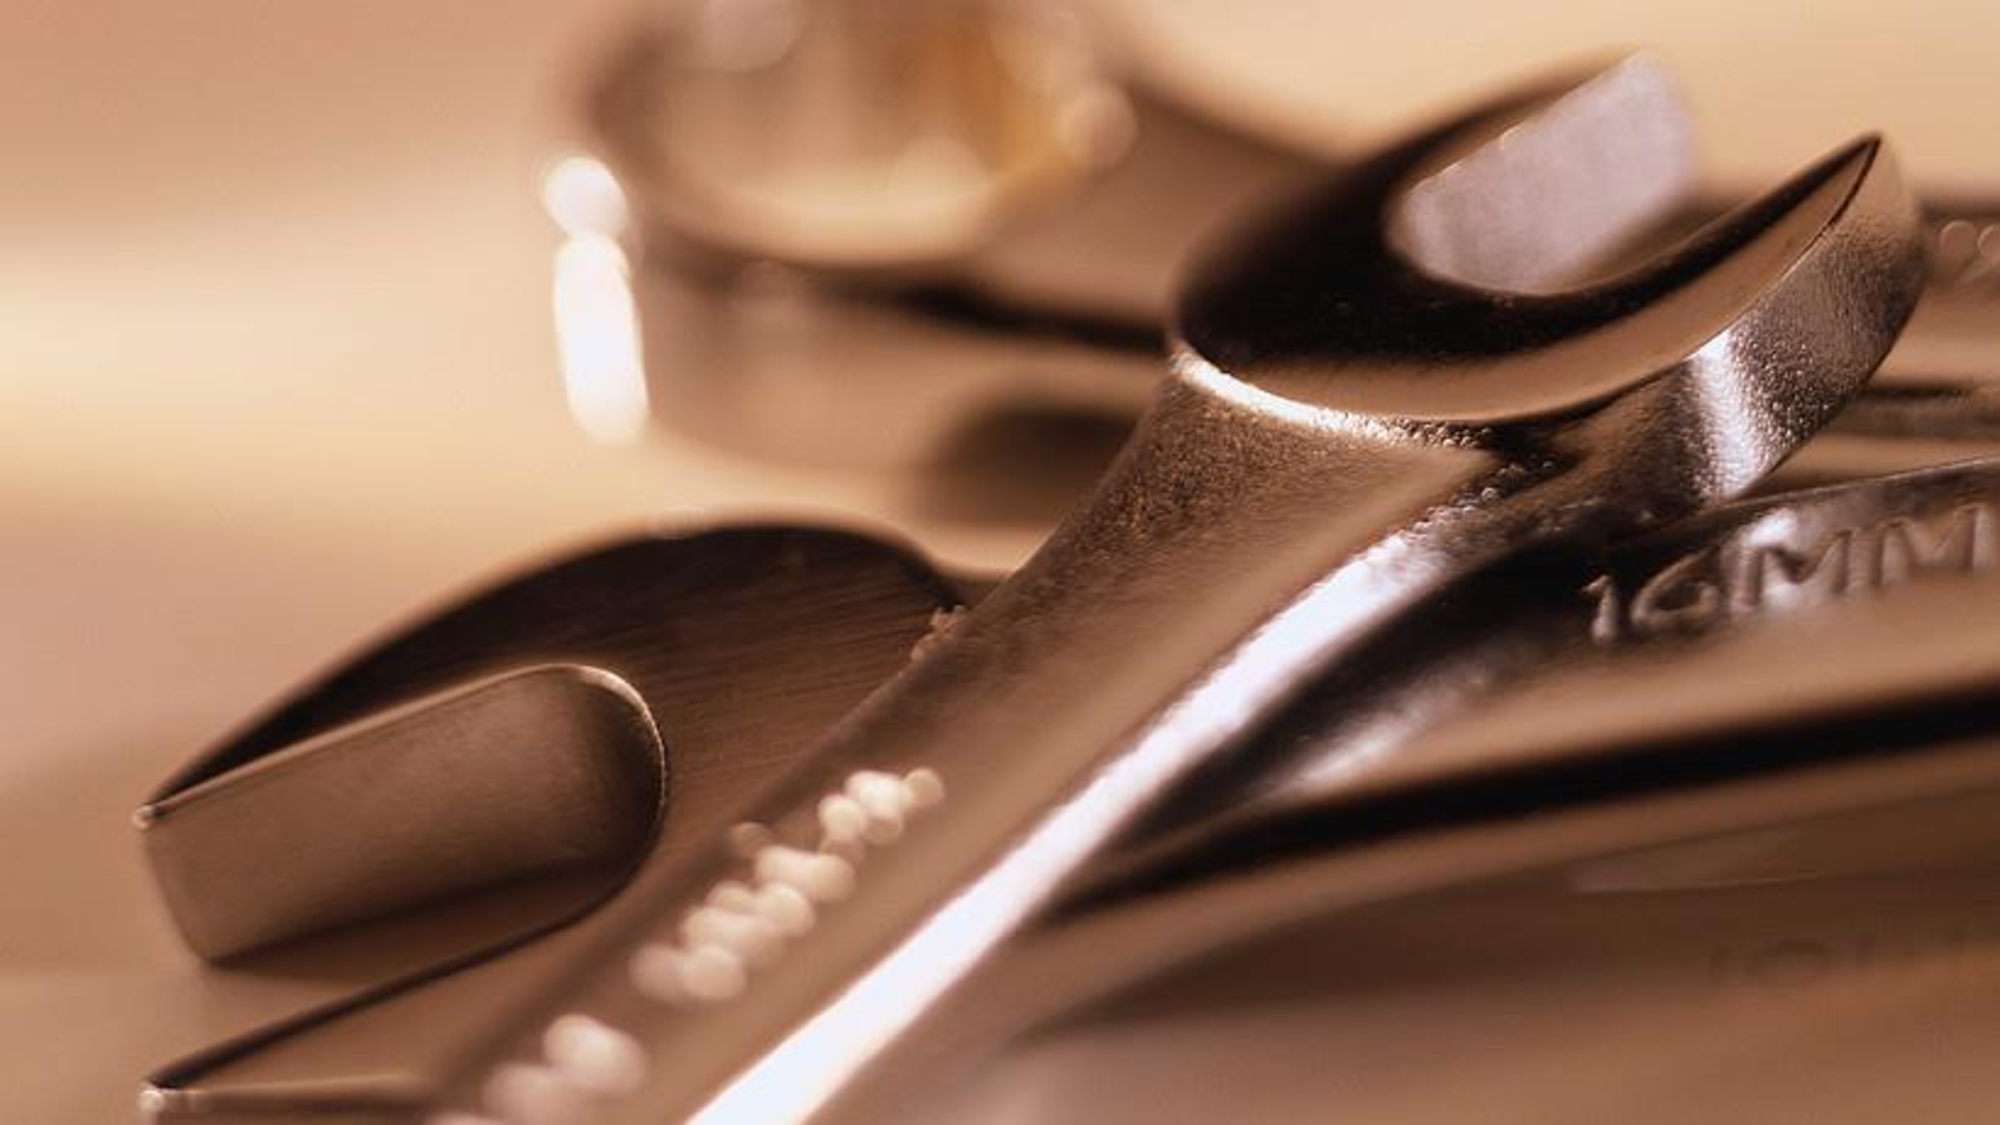
\includegraphics[width=12cm]{Fig/ChangesInManufacturing.pdf}
\caption{製造業におけるニーズとソリューション選択肢の変遷}\label{fig:ChangesInManufacturing}\end{figure}


\subsection{問題の本質の同定}

もともとロボット単体で生産セルを構成するという基本的な考え方は,すでに1980年代の後半に提案されている\cite{Zupancic1988}.当時,人工知能研究もエキスパートシステムと呼ばれる実用化が見られるようになり,バックプロパゲーション則の発見によるニューラルネットワークや,直接法Fuzzy推論則によるFuzzy制御の応用,遺伝的アルゴリズムの応用などが進展しはじめた時代背景とあいまって,生産分野でも,工作機械など熟練者の手に委ねられてきた生産財の知能化研究と実用化が進められてきた.

しかしながら,それらの研究開発成果は,自動化には成功するものの,この手の知的制御システムを
構築するにあたり,熟練作業者モデルを構築するためのシステムの開発,および熟練作業者モデリングの困難さは課題として残ることになった.さらには,1990年代後半から2000年にかけて生産システムの規模が年々大きく複雑化しはじめ,システム構築が属人的技能にとどまっている点も大きな問題となり始めていた\cite{Noda2004}.
2000年代後半になると,産業現場の実務上の問題として,エンジニアリングコストの大きさがシステム構築のボトルネックとなっていることが,はっきりと認識されるようになった.エンジニアリングは,属人的な知識集約作業の典型例であり,リードタイムの長さもコストの一部として計上される.

そこで,著者らの研究グループではこのエンジニアリングコストの削減のため,問題の分析を実施し,本質的な解決策として必要な知能化機能を同定した.これを,第2章で詳報する.

通常,ロボットの知能化というと,外界センサーフードバックにより従来できなかった複雑な動作軌道を実現することに主眼が置かれるが,著者らの研究グループの独創性は,現場のニーズに直接立脚した点にある.
産業用ロボットは生産財である.このため,知能を持った新しいロボットが安全・高速・安定な繰り返し作業を,従来方式となんら変わりなく実現することは大前提である.そのもとで,生産品目切り替えや誤った部品の混入などの大きな外乱に柔軟に対応すること,繰り返し作業への習熟といった自律性を発現する必要がある.
つまり複雑な作業が可能となったとしても動作速度が落ちてしまったり,投資コストが大きくなってしまったりすると,現場では受け入れられない.従来型の生産システムが採用され,極端な場合は作業者を雇い入れるといった解決策が取られることになる.

また,エンジニアリングコストの削減に注目することは,これまでにない視点であり独創性が高い.\cite{robotneeds}%参考文献引用例


\begin{table}[tb]
  \centering
    \caption{値段表}
  \begin{tabular}{|l|c|r||r|} \hline
    メニュー & サイズ & 値段 & カロリー \\ \hline \hline
    牛丼 & 並盛 & 500円 & 600 kcal \\
    牛丼 & 大盛 & 1,000円 & 800 kcal \\
    牛丼 & 特盛 & 1,500円 & 1,000 kcal \\ \hline
  \end{tabular}
\end{table}


\subsection{研究開発のグランドデザインと本論文の主題}

このもとで,知能化技術の要素を開発し,技術プラットフォームとして統合することにした.このことを第3章で詳報する.
そこでは,それぞれの課題の解決のための知能化技術の開発を進めていることを述べる.

研究開発を進めるなかで,人の知能のうち,とりわけ自律性が重要な役割を担っていることがわかったので,製造業向けロボットに自律性を付与する各システムアルゴリズムを開発することにし,これを本論文の主題とした.

まず,人の自律性の最たる特徴の試行錯誤による習熟を,未知の目的関数の最適化問題として定式化して独自の自律システムアルゴリズム「能動型探索アルゴリズム」を提案し,実際のシステムで効果を確認した.また,同種の困難性を持つ問題に対し効果を確認した.これは第4章で詳報する.

次に,自動化システムにおける製品組立作業ではバラ積み状態の部品供給が必ず問題となる.そこで多品種部品のバラ積み供給を実現するシステム設計理論と動作の試行錯誤を実行する「持ち替えグラフアルゴリズム」を提案し,実際の現場で効果を確認した.これは第5章で詳報する.\newpage



\subsection{本論文の構成について}
\noindent
次章以降を,上述した内容に沿って,以下の6つの章で構成する.\\

\noindent
第2章では,自動化システム研究の現状を分析し,課題を明らかにする.\\

\noindent
第3章では,課題を解決するための技術プラットフォーム「自律型セル生産ロボットシステム」の全容について述べる.\\

\noindent
第4章では,課題として重要な自律性の発現について,動作習熟のための自律システムアルゴリズム「能動探索アルゴリズム」について述べる.\\

\noindent
第5章では,おなじく自律性の発現について,バラ積み部品供給のための自律システムアルゴリズム「持ち替えグラフ」について述べる.\\

\noindent
第6章では,実際の製品組立作業を実行するセル生産ロボットシステムを構築して開発技術を検証した結果を報告する.\\

\noindent
第7章で,全体を通じての結論を述べる.\\



\endinput

% for DEBUG % 


% for DEBUG % \setcounter{chapter}{3}
% for DEBUG % 
% !TEX root = thesis.tex
% !TEX encoding = Shift_JIS
% !TEX spellcheck = none


\section{序論}
\subsection{はじめに}

本論文の主題は,第4章と第5章に示す自律システムアルゴリズムである.
同アルゴリズムの研究開発に辿り着くまでには,各時代の要請の変遷とそれを解決するための研究開発の経緯があった.
そこで,なぜ3章以降の開発が必要になったかを明確に定義づけるため,
解説論文的な記述にはなるが,本章と第2章でこれらを示すことにする.

第3章ではそれらを踏まえて開始した,自律型セル生産ロボットシステム技術プラットフォームの
開発プロジェクトの概要について述べる.これはオープンイノベーションを活用した数十人規模の
一大プロジェクトであった.

第4章および第5章で,同プラットフォームに対する要求のなかで最も困難性の高い課題を解決するための
自律システムアルゴリズムについて報告する.




\subsection{背景と動機}

生産人口の減少は,まず日本が,その後,世界が必ず直面する構造問題である.これに対し,あらゆる分野に自動化を万遍なく普及させることが,安全安心で豊かな未来を維持発展させる方法の一つとなる.

製造業分野に目を向けると,動力を利用するようなった産業革命以来,生産を自動化して安価で高品質な製品を大量にライン生産することで,豊かな生活の実現に貢献してきた.
ライン生産方式というソリューションは,設備投資コスト・運用コストを長い期間をかけて回収することが前提であり,つまり概してそれらのコストは大きくなるデメリットがあるものの,一度構築して安定して運用できるようになれば,高速で安定した生産の自動化を維持することにより,同じ品質の製品を大量に製造することができることがメリットとなる.ライン生産方式に投入されるロボットは,この目的のためにその機能を最適設計され,製造されている.そのようなロボットの行動計画は,ライン構築技術者がライン構築時に知恵を絞って設計し,生産活動開始後は,ロボットはあらかじめ定められた単純な位置決め動作を高速に繰り返すことのみに特化していた.これは,動物が条件反射で運動していることに相当する.1990年代にはいると,二次元ビジョンセンサが普及しはじめ,多少の位置ずれをロボット自ら修正する意味での知能化が実用化したが,やはり単純な位置決め動作を高速に繰り返すことに主眼が置かれていて生産ラインの一部への導入にとどまっていた.

2000年代に入ると市場ニーズが多様化しはじめ,短期間のうちに生産機種を切り替える必要が生じた.
このような状況の変化に低コストで柔軟に実施できる人セル生産方式と呼ばれるソリューションが新たな選択肢として注目され,同方式をフル活用したEMS(
\underline{E}lectronics
\underline{M}anufacturing
\underline{S}ervice)事業者も躍進した.
しかし,セル生産方式の生産能力はライン方式に比して低位である.さらには作業者の熟練度に依存する品質のばらつきが直近の課題として取り沙汰されるようになり,これらを解決するために労働者の選抜制をとるなどの方法が取られた.さらには景気の変動に応じて雇用を増減することなどもあわせて,これらの非人道な対応が社会問題となった.また,このような人手をあてにした方式は中長期的には生産人口減少の影響と無縁ではない.

やがて2000年代後半になると,冒頭で述べた生産人口減少問題がようやく人口に膾炙するようになり,
実際に統計的にも日本の人口が減少しはじめ,少子高齢化,生産人口の減少が現実のものとして議論されるようになった.同時に新興国の工業化と市場化の進展により国際競争が激化し,半導体製品・電気電子製品の設計製造技術の革新,景気変動・為替レートの変容・市場ニーズの激変に対応するための市場オフショア生産と地産地消と生産拠点国内回帰の選択の混乱,および市場のグローバル化といった複雑な事象が急速に同時進行したことで,次世代のものつくりの方式が求められ始めていたのが,この2000年代後半の展開であった.

著者らの研究グループでは複雑な状況に対応するためのソリューションの選択肢を増やすため,2006年に新規の研究プロジェクトをスタートさせ,ライン方式,人セル方式,それぞれのメリットを集めたセル生産ロボット方式の実用化を目指すことにした.
ライン生産方式は上述のごとく品種の生産期間は長いことを前提とし少品種大量生産のために最適化され,生産される品質も安定している.ライン生産のなかで産業ロボットは,ワークや治具をピック・アンド・プレースする単純作業に投入されていた.一方,人セル生産方式は生産品種の切り替えが数か月未満で行われることを前提とし,生産速度よりも機種切り替えコストを重視した最適化の結果となっていた.生産速度はラインに比して低いがセルを並列化することで補うという考え方であった.品質は人に依存してばらつきが大きくなっていた.

これに対し,本研究で提案するセル生産ロボット方式では,品種切り替えは迅速,生産速度はそこそこだが品質は安定しているという良いところ取りを目指し,生産速度の増減は,セルの並列数を変化させることで対応しようという概念となる.
ここまで述べてきたことを概念的に図\ref{fig:ChangesInManufacturing}にまとめる.

\begin{figure}[b]\centering 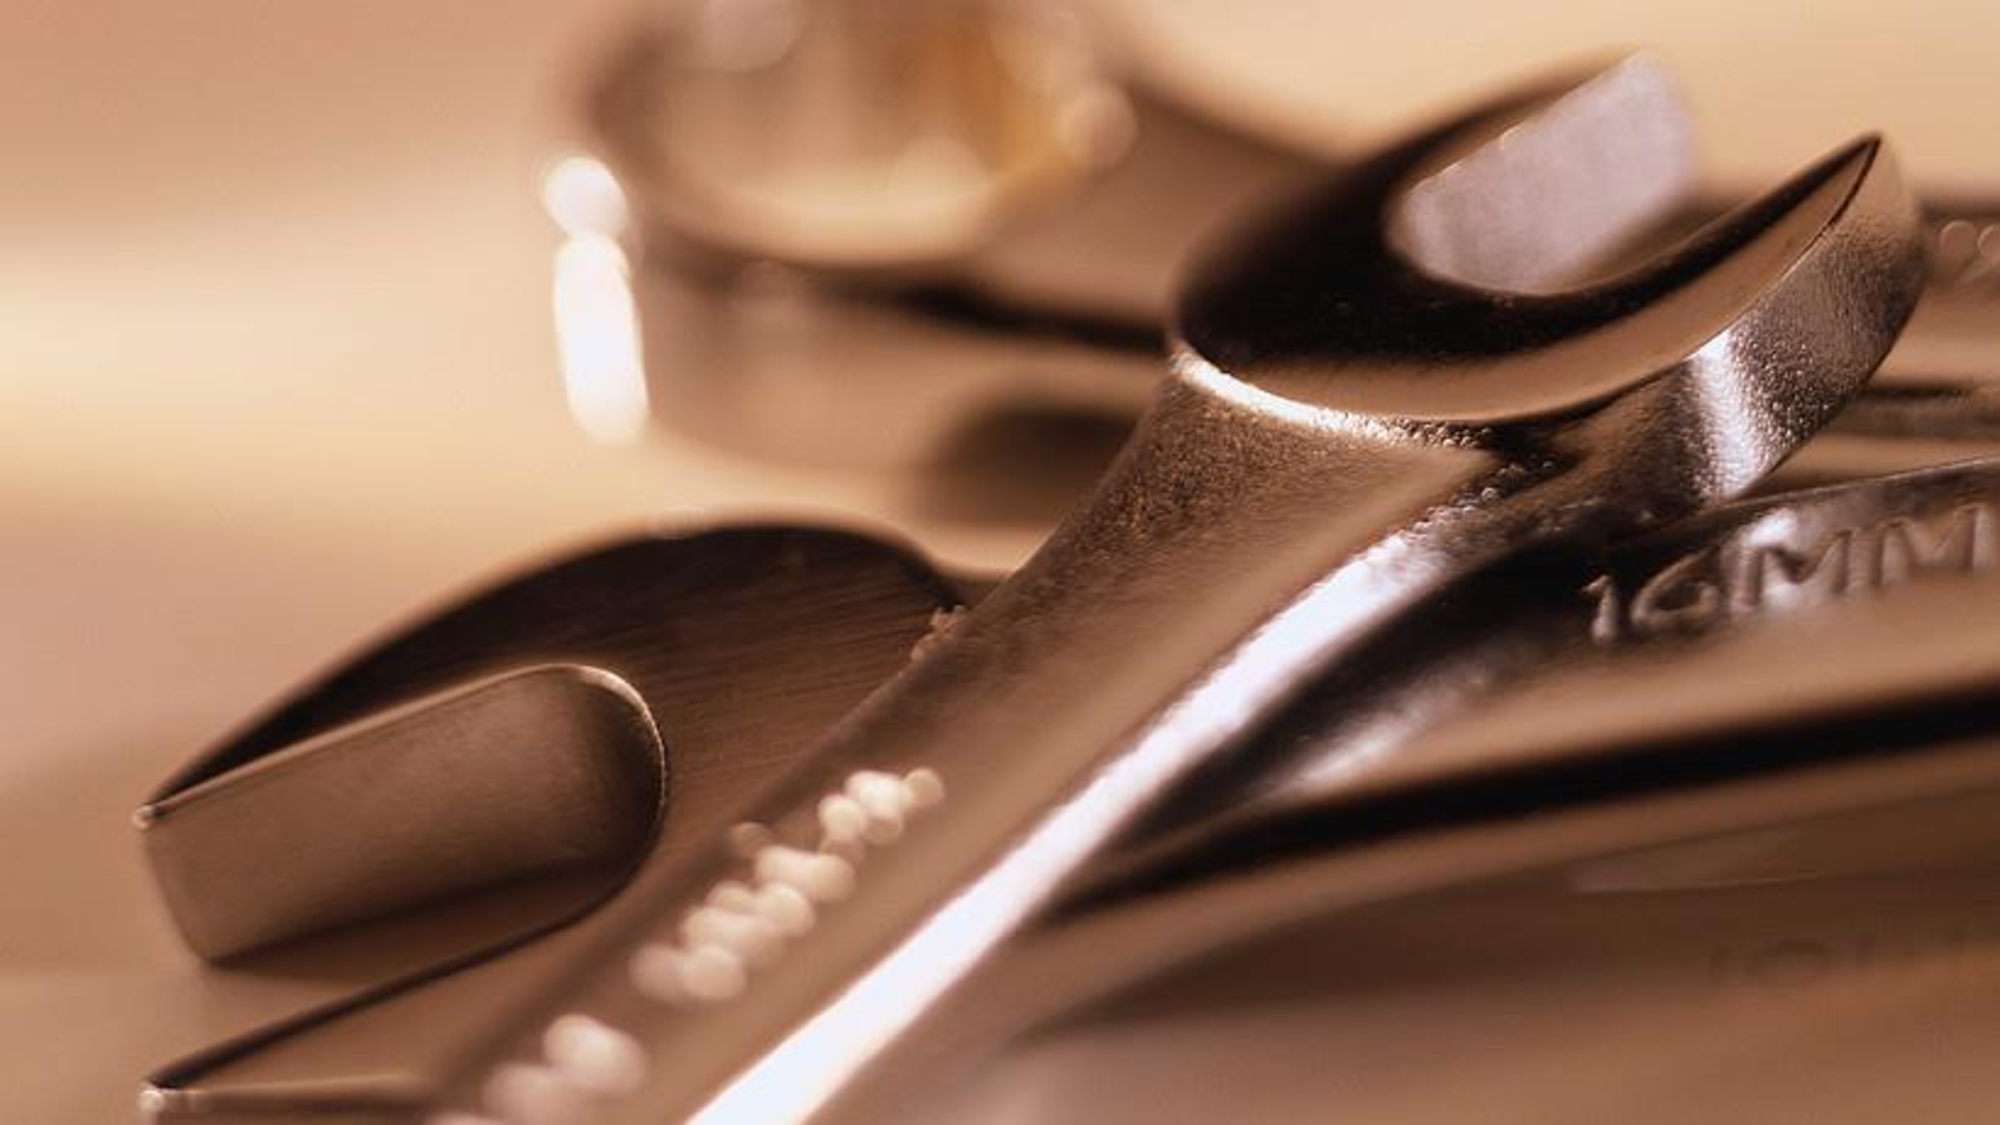
\includegraphics[width=12cm]{Fig/ChangesInManufacturing.pdf}
\caption{製造業におけるニーズとソリューション選択肢の変遷}\label{fig:ChangesInManufacturing}\end{figure}


\subsection{問題の本質の同定}

もともとロボット単体で生産セルを構成するという基本的な考え方は,すでに1980年代の後半に提案されている\cite{Zupancic1988}.当時,人工知能研究もエキスパートシステムと呼ばれる実用化が見られるようになり,バックプロパゲーション則の発見によるニューラルネットワークや,直接法Fuzzy推論則によるFuzzy制御の応用,遺伝的アルゴリズムの応用などが進展しはじめた時代背景とあいまって,生産分野でも,工作機械など熟練者の手に委ねられてきた生産財の知能化研究と実用化が進められてきた.

しかしながら,それらの研究開発成果は,自動化には成功するものの,この手の知的制御システムを
構築するにあたり,熟練作業者モデルを構築するためのシステムの開発,および熟練作業者モデリングの困難さは課題として残ることになった.さらには,1990年代後半から2000年にかけて生産システムの規模が年々大きく複雑化しはじめ,システム構築が属人的技能にとどまっている点も大きな問題となり始めていた\cite{Noda2004}.
2000年代後半になると,産業現場の実務上の問題として,エンジニアリングコストの大きさがシステム構築のボトルネックとなっていることが,はっきりと認識されるようになった.エンジニアリングは,属人的な知識集約作業の典型例であり,リードタイムの長さもコストの一部として計上される.

そこで,著者らの研究グループではこのエンジニアリングコストの削減のため,問題の分析を実施し,本質的な解決策として必要な知能化機能を同定した.これを,第2章で詳報する.

通常,ロボットの知能化というと,外界センサーフードバックにより従来できなかった複雑な動作軌道を実現することに主眼が置かれるが,著者らの研究グループの独創性は,現場のニーズに直接立脚した点にある.
産業用ロボットは生産財である.このため,知能を持った新しいロボットが安全・高速・安定な繰り返し作業を,従来方式となんら変わりなく実現することは大前提である.そのもとで,生産品目切り替えや誤った部品の混入などの大きな外乱に柔軟に対応すること,繰り返し作業への習熟といった自律性を発現する必要がある.
つまり複雑な作業が可能となったとしても動作速度が落ちてしまったり,投資コストが大きくなってしまったりすると,現場では受け入れられない.従来型の生産システムが採用され,極端な場合は作業者を雇い入れるといった解決策が取られることになる.

また,エンジニアリングコストの削減に注目することは,これまでにない視点であり独創性が高い.\cite{robotneeds}%参考文献引用例


\begin{table}[tb]
  \centering
    \caption{値段表}
  \begin{tabular}{|l|c|r||r|} \hline
    メニュー & サイズ & 値段 & カロリー \\ \hline \hline
    牛丼 & 並盛 & 500円 & 600 kcal \\
    牛丼 & 大盛 & 1,000円 & 800 kcal \\
    牛丼 & 特盛 & 1,500円 & 1,000 kcal \\ \hline
  \end{tabular}
\end{table}


\subsection{研究開発のグランドデザインと本論文の主題}

このもとで,知能化技術の要素を開発し,技術プラットフォームとして統合することにした.このことを第3章で詳報する.
そこでは,それぞれの課題の解決のための知能化技術の開発を進めていることを述べる.

研究開発を進めるなかで,人の知能のうち,とりわけ自律性が重要な役割を担っていることがわかったので,製造業向けロボットに自律性を付与する各システムアルゴリズムを開発することにし,これを本論文の主題とした.

まず,人の自律性の最たる特徴の試行錯誤による習熟を,未知の目的関数の最適化問題として定式化して独自の自律システムアルゴリズム「能動型探索アルゴリズム」を提案し,実際のシステムで効果を確認した.また,同種の困難性を持つ問題に対し効果を確認した.これは第4章で詳報する.

次に,自動化システムにおける製品組立作業ではバラ積み状態の部品供給が必ず問題となる.そこで多品種部品のバラ積み供給を実現するシステム設計理論と動作の試行錯誤を実行する「持ち替えグラフアルゴリズム」を提案し,実際の現場で効果を確認した.これは第5章で詳報する.\newpage



\subsection{本論文の構成について}
\noindent
次章以降を,上述した内容に沿って,以下の6つの章で構成する.\\

\noindent
第2章では,自動化システム研究の現状を分析し,課題を明らかにする.\\

\noindent
第3章では,課題を解決するための技術プラットフォーム「自律型セル生産ロボットシステム」の全容について述べる.\\

\noindent
第4章では,課題として重要な自律性の発現について,動作習熟のための自律システムアルゴリズム「能動探索アルゴリズム」について述べる.\\

\noindent
第5章では,おなじく自律性の発現について,バラ積み部品供給のための自律システムアルゴリズム「持ち替えグラフ」について述べる.\\

\noindent
第6章では,実際の製品組立作業を実行するセル生産ロボットシステムを構築して開発技術を検証した結果を報告する.\\

\noindent
第7章で,全体を通じての結論を述べる.\\



\endinput

% for DEBUG % 
% !TEX root = thesis.tex
% !TEX encoding = Shift_JIS
% !TEX spellcheck = none


\section{序論}
\subsection{はじめに}

本論文の主題は,第4章と第5章に示す自律システムアルゴリズムである.
同アルゴリズムの研究開発に辿り着くまでには,各時代の要請の変遷とそれを解決するための研究開発の経緯があった.
そこで,なぜ3章以降の開発が必要になったかを明確に定義づけるため,
解説論文的な記述にはなるが,本章と第2章でこれらを示すことにする.

第3章ではそれらを踏まえて開始した,自律型セル生産ロボットシステム技術プラットフォームの
開発プロジェクトの概要について述べる.これはオープンイノベーションを活用した数十人規模の
一大プロジェクトであった.

第4章および第5章で,同プラットフォームに対する要求のなかで最も困難性の高い課題を解決するための
自律システムアルゴリズムについて報告する.




\subsection{背景と動機}

生産人口の減少は,まず日本が,その後,世界が必ず直面する構造問題である.これに対し,あらゆる分野に自動化を万遍なく普及させることが,安全安心で豊かな未来を維持発展させる方法の一つとなる.

製造業分野に目を向けると,動力を利用するようなった産業革命以来,生産を自動化して安価で高品質な製品を大量にライン生産することで,豊かな生活の実現に貢献してきた.
ライン生産方式というソリューションは,設備投資コスト・運用コストを長い期間をかけて回収することが前提であり,つまり概してそれらのコストは大きくなるデメリットがあるものの,一度構築して安定して運用できるようになれば,高速で安定した生産の自動化を維持することにより,同じ品質の製品を大量に製造することができることがメリットとなる.ライン生産方式に投入されるロボットは,この目的のためにその機能を最適設計され,製造されている.そのようなロボットの行動計画は,ライン構築技術者がライン構築時に知恵を絞って設計し,生産活動開始後は,ロボットはあらかじめ定められた単純な位置決め動作を高速に繰り返すことのみに特化していた.これは,動物が条件反射で運動していることに相当する.1990年代にはいると,二次元ビジョンセンサが普及しはじめ,多少の位置ずれをロボット自ら修正する意味での知能化が実用化したが,やはり単純な位置決め動作を高速に繰り返すことに主眼が置かれていて生産ラインの一部への導入にとどまっていた.

2000年代に入ると市場ニーズが多様化しはじめ,短期間のうちに生産機種を切り替える必要が生じた.
このような状況の変化に低コストで柔軟に実施できる人セル生産方式と呼ばれるソリューションが新たな選択肢として注目され,同方式をフル活用したEMS(
\underline{E}lectronics
\underline{M}anufacturing
\underline{S}ervice)事業者も躍進した.
しかし,セル生産方式の生産能力はライン方式に比して低位である.さらには作業者の熟練度に依存する品質のばらつきが直近の課題として取り沙汰されるようになり,これらを解決するために労働者の選抜制をとるなどの方法が取られた.さらには景気の変動に応じて雇用を増減することなどもあわせて,これらの非人道な対応が社会問題となった.また,このような人手をあてにした方式は中長期的には生産人口減少の影響と無縁ではない.

やがて2000年代後半になると,冒頭で述べた生産人口減少問題がようやく人口に膾炙するようになり,
実際に統計的にも日本の人口が減少しはじめ,少子高齢化,生産人口の減少が現実のものとして議論されるようになった.同時に新興国の工業化と市場化の進展により国際競争が激化し,半導体製品・電気電子製品の設計製造技術の革新,景気変動・為替レートの変容・市場ニーズの激変に対応するための市場オフショア生産と地産地消と生産拠点国内回帰の選択の混乱,および市場のグローバル化といった複雑な事象が急速に同時進行したことで,次世代のものつくりの方式が求められ始めていたのが,この2000年代後半の展開であった.

著者らの研究グループでは複雑な状況に対応するためのソリューションの選択肢を増やすため,2006年に新規の研究プロジェクトをスタートさせ,ライン方式,人セル方式,それぞれのメリットを集めたセル生産ロボット方式の実用化を目指すことにした.
ライン生産方式は上述のごとく品種の生産期間は長いことを前提とし少品種大量生産のために最適化され,生産される品質も安定している.ライン生産のなかで産業ロボットは,ワークや治具をピック・アンド・プレースする単純作業に投入されていた.一方,人セル生産方式は生産品種の切り替えが数か月未満で行われることを前提とし,生産速度よりも機種切り替えコストを重視した最適化の結果となっていた.生産速度はラインに比して低いがセルを並列化することで補うという考え方であった.品質は人に依存してばらつきが大きくなっていた.

これに対し,本研究で提案するセル生産ロボット方式では,品種切り替えは迅速,生産速度はそこそこだが品質は安定しているという良いところ取りを目指し,生産速度の増減は,セルの並列数を変化させることで対応しようという概念となる.
ここまで述べてきたことを概念的に図\ref{fig:ChangesInManufacturing}にまとめる.

\begin{figure}[b]\centering 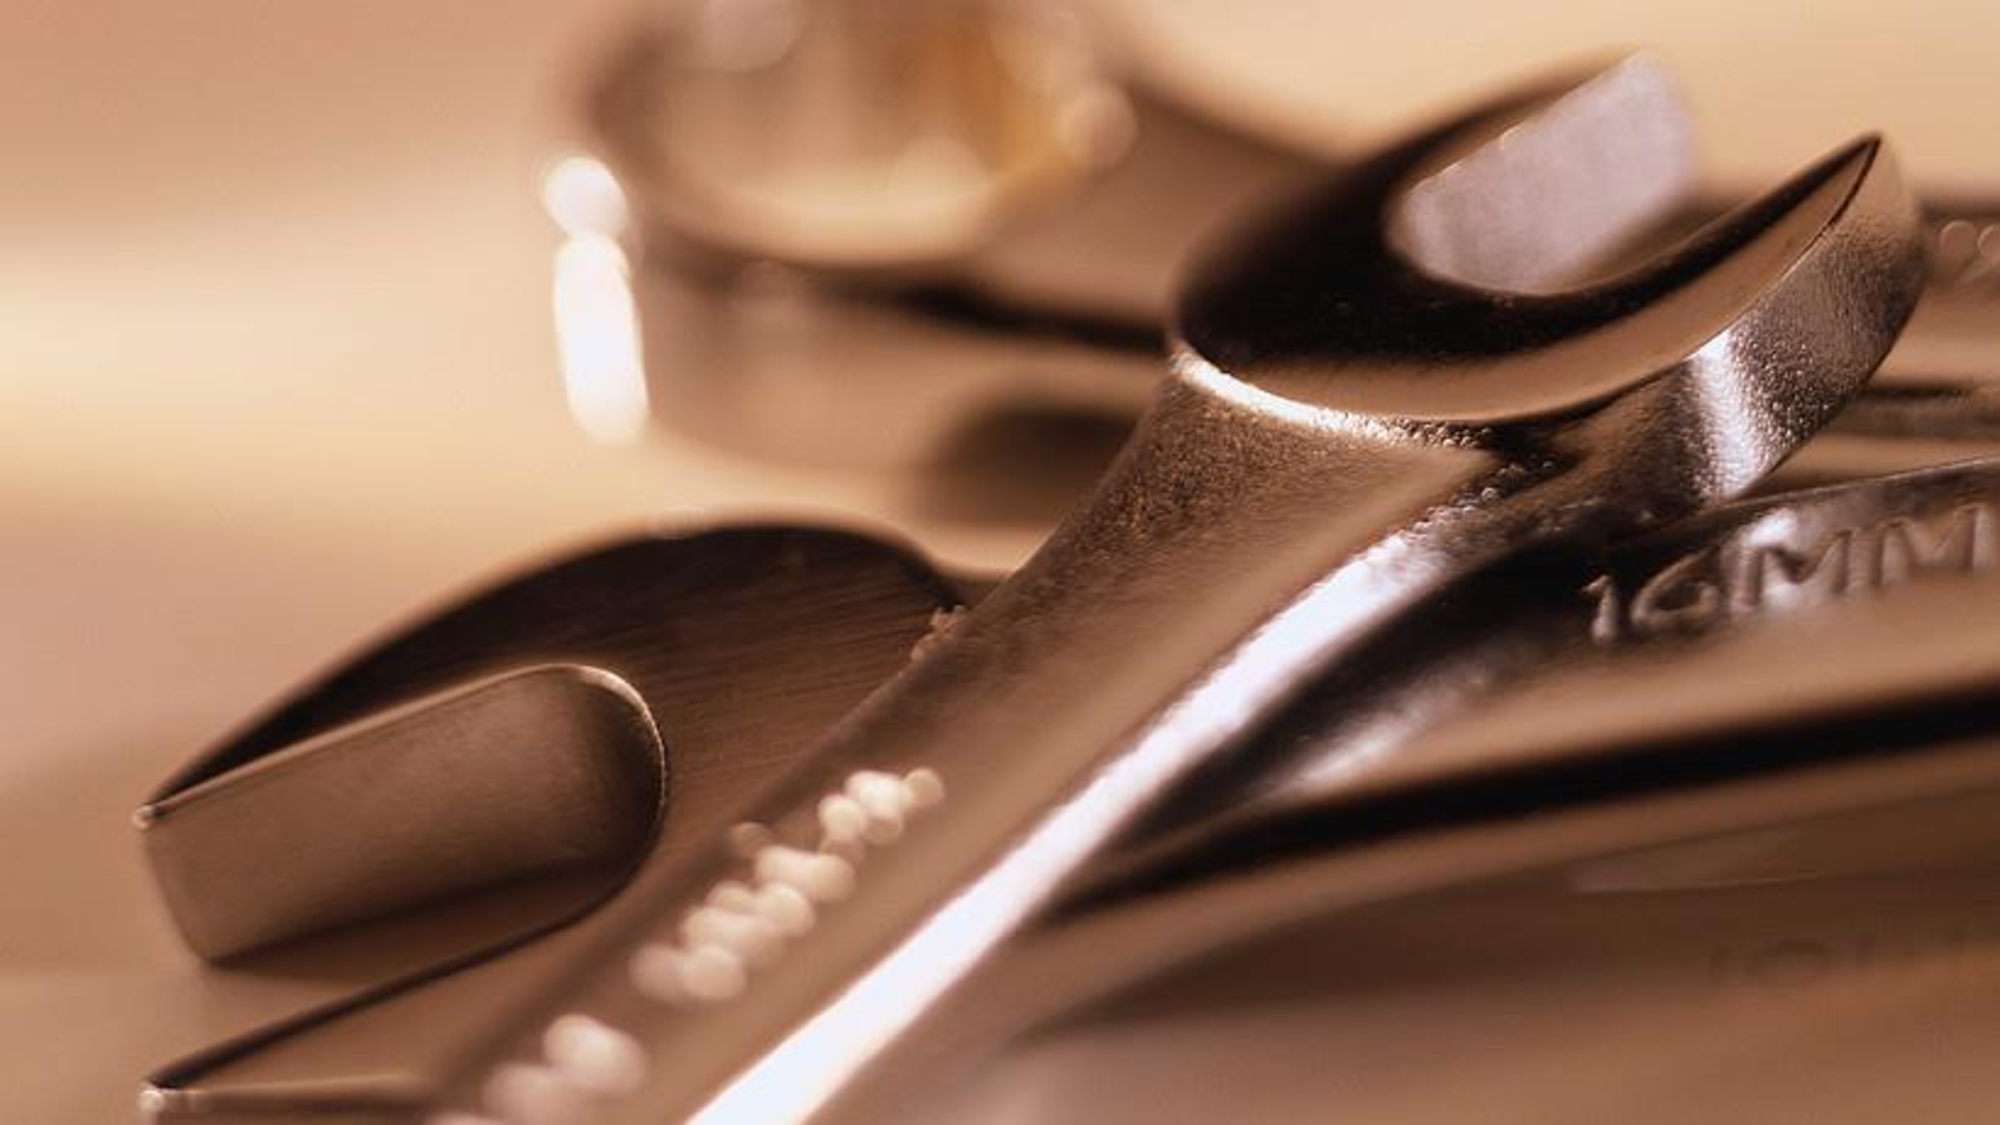
\includegraphics[width=12cm]{Fig/ChangesInManufacturing.pdf}
\caption{製造業におけるニーズとソリューション選択肢の変遷}\label{fig:ChangesInManufacturing}\end{figure}


\subsection{問題の本質の同定}

もともとロボット単体で生産セルを構成するという基本的な考え方は,すでに1980年代の後半に提案されている\cite{Zupancic1988}.当時,人工知能研究もエキスパートシステムと呼ばれる実用化が見られるようになり,バックプロパゲーション則の発見によるニューラルネットワークや,直接法Fuzzy推論則によるFuzzy制御の応用,遺伝的アルゴリズムの応用などが進展しはじめた時代背景とあいまって,生産分野でも,工作機械など熟練者の手に委ねられてきた生産財の知能化研究と実用化が進められてきた.

しかしながら,それらの研究開発成果は,自動化には成功するものの,この手の知的制御システムを
構築するにあたり,熟練作業者モデルを構築するためのシステムの開発,および熟練作業者モデリングの困難さは課題として残ることになった.さらには,1990年代後半から2000年にかけて生産システムの規模が年々大きく複雑化しはじめ,システム構築が属人的技能にとどまっている点も大きな問題となり始めていた\cite{Noda2004}.
2000年代後半になると,産業現場の実務上の問題として,エンジニアリングコストの大きさがシステム構築のボトルネックとなっていることが,はっきりと認識されるようになった.エンジニアリングは,属人的な知識集約作業の典型例であり,リードタイムの長さもコストの一部として計上される.

そこで,著者らの研究グループではこのエンジニアリングコストの削減のため,問題の分析を実施し,本質的な解決策として必要な知能化機能を同定した.これを,第2章で詳報する.

通常,ロボットの知能化というと,外界センサーフードバックにより従来できなかった複雑な動作軌道を実現することに主眼が置かれるが,著者らの研究グループの独創性は,現場のニーズに直接立脚した点にある.
産業用ロボットは生産財である.このため,知能を持った新しいロボットが安全・高速・安定な繰り返し作業を,従来方式となんら変わりなく実現することは大前提である.そのもとで,生産品目切り替えや誤った部品の混入などの大きな外乱に柔軟に対応すること,繰り返し作業への習熟といった自律性を発現する必要がある.
つまり複雑な作業が可能となったとしても動作速度が落ちてしまったり,投資コストが大きくなってしまったりすると,現場では受け入れられない.従来型の生産システムが採用され,極端な場合は作業者を雇い入れるといった解決策が取られることになる.

また,エンジニアリングコストの削減に注目することは,これまでにない視点であり独創性が高い.\cite{robotneeds}%参考文献引用例


\begin{table}[tb]
  \centering
    \caption{値段表}
  \begin{tabular}{|l|c|r||r|} \hline
    メニュー & サイズ & 値段 & カロリー \\ \hline \hline
    牛丼 & 並盛 & 500円 & 600 kcal \\
    牛丼 & 大盛 & 1,000円 & 800 kcal \\
    牛丼 & 特盛 & 1,500円 & 1,000 kcal \\ \hline
  \end{tabular}
\end{table}


\subsection{研究開発のグランドデザインと本論文の主題}

このもとで,知能化技術の要素を開発し,技術プラットフォームとして統合することにした.このことを第3章で詳報する.
そこでは,それぞれの課題の解決のための知能化技術の開発を進めていることを述べる.

研究開発を進めるなかで,人の知能のうち,とりわけ自律性が重要な役割を担っていることがわかったので,製造業向けロボットに自律性を付与する各システムアルゴリズムを開発することにし,これを本論文の主題とした.

まず,人の自律性の最たる特徴の試行錯誤による習熟を,未知の目的関数の最適化問題として定式化して独自の自律システムアルゴリズム「能動型探索アルゴリズム」を提案し,実際のシステムで効果を確認した.また,同種の困難性を持つ問題に対し効果を確認した.これは第4章で詳報する.

次に,自動化システムにおける製品組立作業ではバラ積み状態の部品供給が必ず問題となる.そこで多品種部品のバラ積み供給を実現するシステム設計理論と動作の試行錯誤を実行する「持ち替えグラフアルゴリズム」を提案し,実際の現場で効果を確認した.これは第5章で詳報する.\newpage



\subsection{本論文の構成について}
\noindent
次章以降を,上述した内容に沿って,以下の6つの章で構成する.\\

\noindent
第2章では,自動化システム研究の現状を分析し,課題を明らかにする.\\

\noindent
第3章では,課題を解決するための技術プラットフォーム「自律型セル生産ロボットシステム」の全容について述べる.\\

\noindent
第4章では,課題として重要な自律性の発現について,動作習熟のための自律システムアルゴリズム「能動探索アルゴリズム」について述べる.\\

\noindent
第5章では,おなじく自律性の発現について,バラ積み部品供給のための自律システムアルゴリズム「持ち替えグラフ」について述べる.\\

\noindent
第6章では,実際の製品組立作業を実行するセル生産ロボットシステムを構築して開発技術を検証した結果を報告する.\\

\noindent
第7章で,全体を通じての結論を述べる.\\



\endinput

% for DEBUG % 


% for DEBUG % \setcounter{chapter}{4}
% for DEBUG % 
% !TEX root = thesis.tex
% !TEX encoding = Shift_JIS
% !TEX spellcheck = none


\section{序論}
\subsection{はじめに}

本論文の主題は,第4章と第5章に示す自律システムアルゴリズムである.
同アルゴリズムの研究開発に辿り着くまでには,各時代の要請の変遷とそれを解決するための研究開発の経緯があった.
そこで,なぜ3章以降の開発が必要になったかを明確に定義づけるため,
解説論文的な記述にはなるが,本章と第2章でこれらを示すことにする.

第3章ではそれらを踏まえて開始した,自律型セル生産ロボットシステム技術プラットフォームの
開発プロジェクトの概要について述べる.これはオープンイノベーションを活用した数十人規模の
一大プロジェクトであった.

第4章および第5章で,同プラットフォームに対する要求のなかで最も困難性の高い課題を解決するための
自律システムアルゴリズムについて報告する.




\subsection{背景と動機}

生産人口の減少は,まず日本が,その後,世界が必ず直面する構造問題である.これに対し,あらゆる分野に自動化を万遍なく普及させることが,安全安心で豊かな未来を維持発展させる方法の一つとなる.

製造業分野に目を向けると,動力を利用するようなった産業革命以来,生産を自動化して安価で高品質な製品を大量にライン生産することで,豊かな生活の実現に貢献してきた.
ライン生産方式というソリューションは,設備投資コスト・運用コストを長い期間をかけて回収することが前提であり,つまり概してそれらのコストは大きくなるデメリットがあるものの,一度構築して安定して運用できるようになれば,高速で安定した生産の自動化を維持することにより,同じ品質の製品を大量に製造することができることがメリットとなる.ライン生産方式に投入されるロボットは,この目的のためにその機能を最適設計され,製造されている.そのようなロボットの行動計画は,ライン構築技術者がライン構築時に知恵を絞って設計し,生産活動開始後は,ロボットはあらかじめ定められた単純な位置決め動作を高速に繰り返すことのみに特化していた.これは,動物が条件反射で運動していることに相当する.1990年代にはいると,二次元ビジョンセンサが普及しはじめ,多少の位置ずれをロボット自ら修正する意味での知能化が実用化したが,やはり単純な位置決め動作を高速に繰り返すことに主眼が置かれていて生産ラインの一部への導入にとどまっていた.

2000年代に入ると市場ニーズが多様化しはじめ,短期間のうちに生産機種を切り替える必要が生じた.
このような状況の変化に低コストで柔軟に実施できる人セル生産方式と呼ばれるソリューションが新たな選択肢として注目され,同方式をフル活用したEMS(
\underline{E}lectronics
\underline{M}anufacturing
\underline{S}ervice)事業者も躍進した.
しかし,セル生産方式の生産能力はライン方式に比して低位である.さらには作業者の熟練度に依存する品質のばらつきが直近の課題として取り沙汰されるようになり,これらを解決するために労働者の選抜制をとるなどの方法が取られた.さらには景気の変動に応じて雇用を増減することなどもあわせて,これらの非人道な対応が社会問題となった.また,このような人手をあてにした方式は中長期的には生産人口減少の影響と無縁ではない.

やがて2000年代後半になると,冒頭で述べた生産人口減少問題がようやく人口に膾炙するようになり,
実際に統計的にも日本の人口が減少しはじめ,少子高齢化,生産人口の減少が現実のものとして議論されるようになった.同時に新興国の工業化と市場化の進展により国際競争が激化し,半導体製品・電気電子製品の設計製造技術の革新,景気変動・為替レートの変容・市場ニーズの激変に対応するための市場オフショア生産と地産地消と生産拠点国内回帰の選択の混乱,および市場のグローバル化といった複雑な事象が急速に同時進行したことで,次世代のものつくりの方式が求められ始めていたのが,この2000年代後半の展開であった.

著者らの研究グループでは複雑な状況に対応するためのソリューションの選択肢を増やすため,2006年に新規の研究プロジェクトをスタートさせ,ライン方式,人セル方式,それぞれのメリットを集めたセル生産ロボット方式の実用化を目指すことにした.
ライン生産方式は上述のごとく品種の生産期間は長いことを前提とし少品種大量生産のために最適化され,生産される品質も安定している.ライン生産のなかで産業ロボットは,ワークや治具をピック・アンド・プレースする単純作業に投入されていた.一方,人セル生産方式は生産品種の切り替えが数か月未満で行われることを前提とし,生産速度よりも機種切り替えコストを重視した最適化の結果となっていた.生産速度はラインに比して低いがセルを並列化することで補うという考え方であった.品質は人に依存してばらつきが大きくなっていた.

これに対し,本研究で提案するセル生産ロボット方式では,品種切り替えは迅速,生産速度はそこそこだが品質は安定しているという良いところ取りを目指し,生産速度の増減は,セルの並列数を変化させることで対応しようという概念となる.
ここまで述べてきたことを概念的に図\ref{fig:ChangesInManufacturing}にまとめる.

\begin{figure}[b]\centering 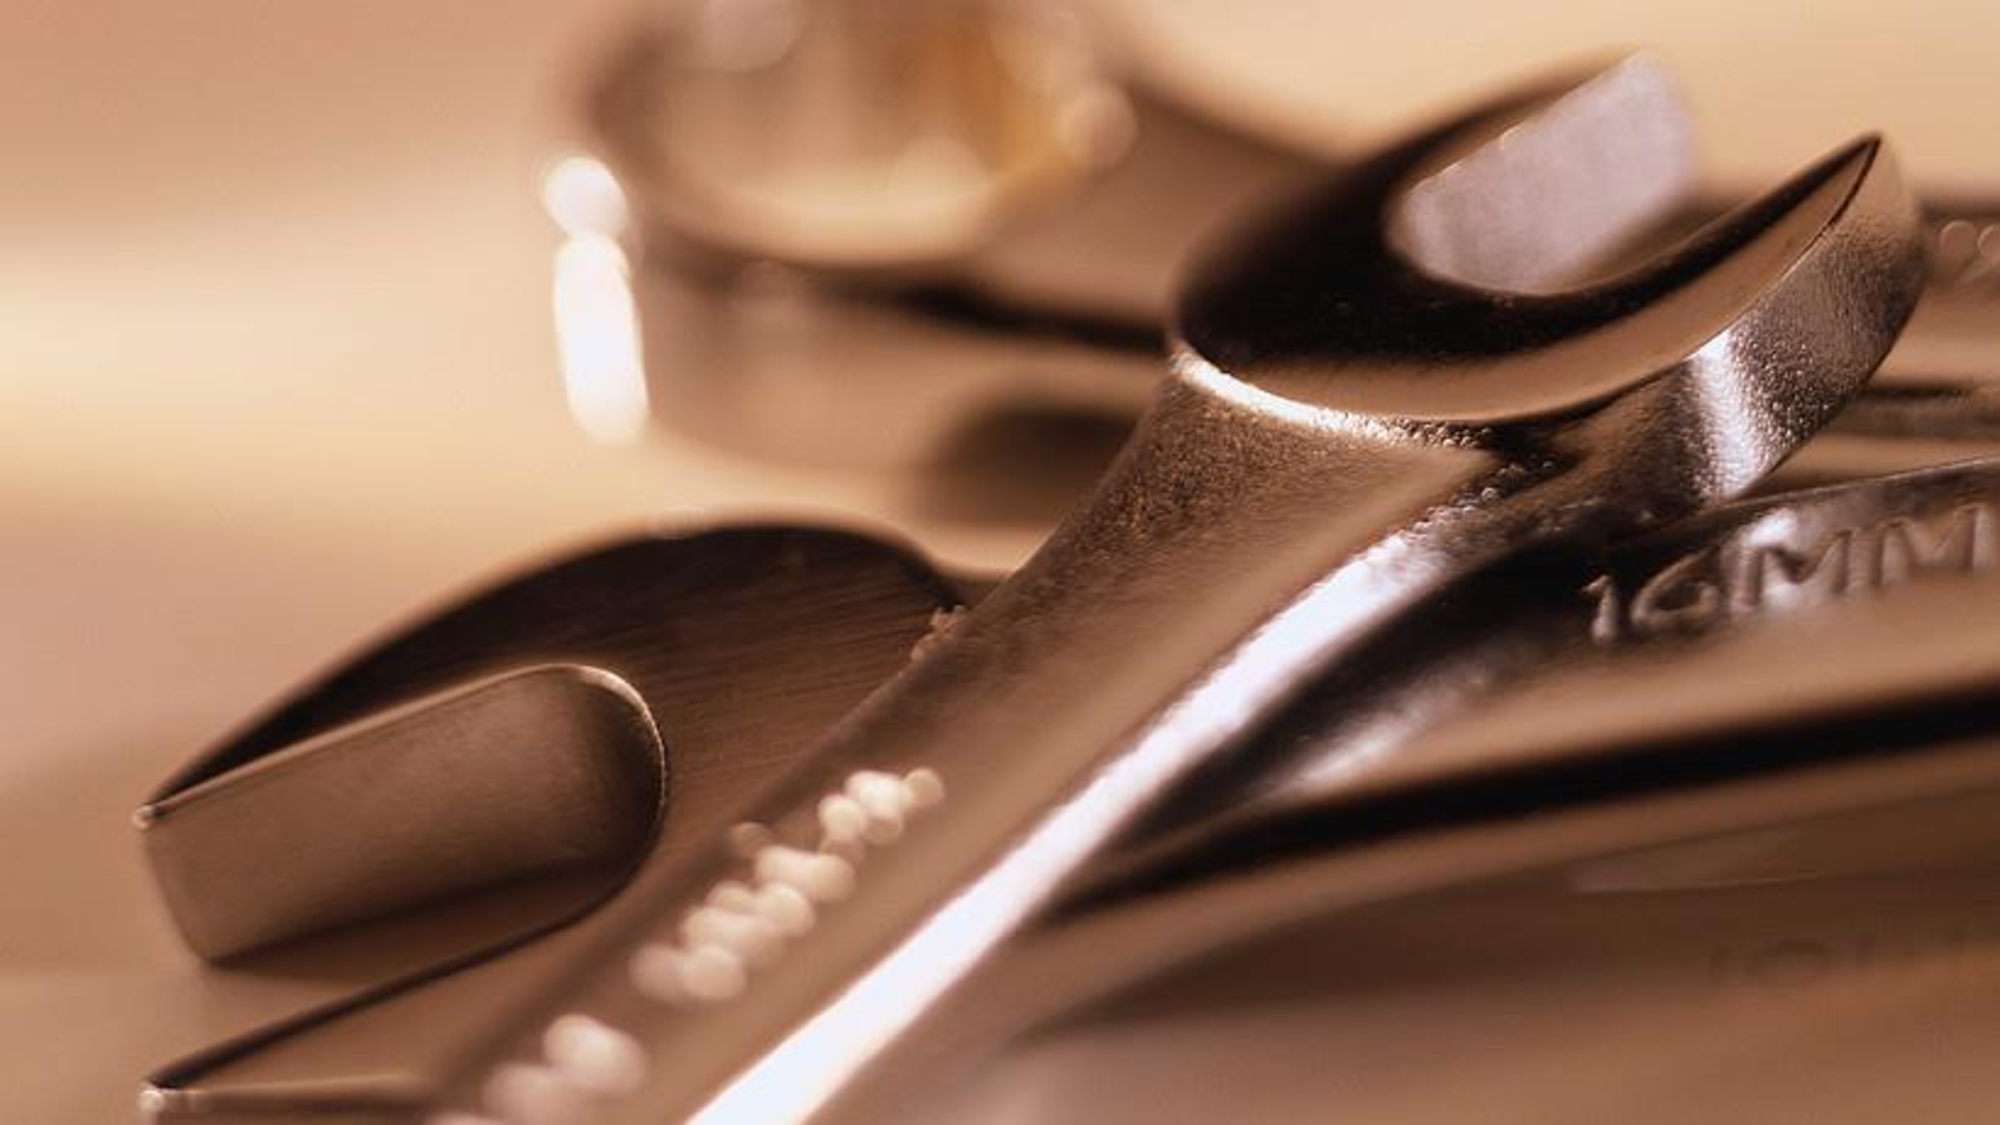
\includegraphics[width=12cm]{Fig/ChangesInManufacturing.pdf}
\caption{製造業におけるニーズとソリューション選択肢の変遷}\label{fig:ChangesInManufacturing}\end{figure}


\subsection{問題の本質の同定}

もともとロボット単体で生産セルを構成するという基本的な考え方は,すでに1980年代の後半に提案されている\cite{Zupancic1988}.当時,人工知能研究もエキスパートシステムと呼ばれる実用化が見られるようになり,バックプロパゲーション則の発見によるニューラルネットワークや,直接法Fuzzy推論則によるFuzzy制御の応用,遺伝的アルゴリズムの応用などが進展しはじめた時代背景とあいまって,生産分野でも,工作機械など熟練者の手に委ねられてきた生産財の知能化研究と実用化が進められてきた.

しかしながら,それらの研究開発成果は,自動化には成功するものの,この手の知的制御システムを
構築するにあたり,熟練作業者モデルを構築するためのシステムの開発,および熟練作業者モデリングの困難さは課題として残ることになった.さらには,1990年代後半から2000年にかけて生産システムの規模が年々大きく複雑化しはじめ,システム構築が属人的技能にとどまっている点も大きな問題となり始めていた\cite{Noda2004}.
2000年代後半になると,産業現場の実務上の問題として,エンジニアリングコストの大きさがシステム構築のボトルネックとなっていることが,はっきりと認識されるようになった.エンジニアリングは,属人的な知識集約作業の典型例であり,リードタイムの長さもコストの一部として計上される.

そこで,著者らの研究グループではこのエンジニアリングコストの削減のため,問題の分析を実施し,本質的な解決策として必要な知能化機能を同定した.これを,第2章で詳報する.

通常,ロボットの知能化というと,外界センサーフードバックにより従来できなかった複雑な動作軌道を実現することに主眼が置かれるが,著者らの研究グループの独創性は,現場のニーズに直接立脚した点にある.
産業用ロボットは生産財である.このため,知能を持った新しいロボットが安全・高速・安定な繰り返し作業を,従来方式となんら変わりなく実現することは大前提である.そのもとで,生産品目切り替えや誤った部品の混入などの大きな外乱に柔軟に対応すること,繰り返し作業への習熟といった自律性を発現する必要がある.
つまり複雑な作業が可能となったとしても動作速度が落ちてしまったり,投資コストが大きくなってしまったりすると,現場では受け入れられない.従来型の生産システムが採用され,極端な場合は作業者を雇い入れるといった解決策が取られることになる.

また,エンジニアリングコストの削減に注目することは,これまでにない視点であり独創性が高い.\cite{robotneeds}%参考文献引用例


\begin{table}[tb]
  \centering
    \caption{値段表}
  \begin{tabular}{|l|c|r||r|} \hline
    メニュー & サイズ & 値段 & カロリー \\ \hline \hline
    牛丼 & 並盛 & 500円 & 600 kcal \\
    牛丼 & 大盛 & 1,000円 & 800 kcal \\
    牛丼 & 特盛 & 1,500円 & 1,000 kcal \\ \hline
  \end{tabular}
\end{table}


\subsection{研究開発のグランドデザインと本論文の主題}

このもとで,知能化技術の要素を開発し,技術プラットフォームとして統合することにした.このことを第3章で詳報する.
そこでは,それぞれの課題の解決のための知能化技術の開発を進めていることを述べる.

研究開発を進めるなかで,人の知能のうち,とりわけ自律性が重要な役割を担っていることがわかったので,製造業向けロボットに自律性を付与する各システムアルゴリズムを開発することにし,これを本論文の主題とした.

まず,人の自律性の最たる特徴の試行錯誤による習熟を,未知の目的関数の最適化問題として定式化して独自の自律システムアルゴリズム「能動型探索アルゴリズム」を提案し,実際のシステムで効果を確認した.また,同種の困難性を持つ問題に対し効果を確認した.これは第4章で詳報する.

次に,自動化システムにおける製品組立作業ではバラ積み状態の部品供給が必ず問題となる.そこで多品種部品のバラ積み供給を実現するシステム設計理論と動作の試行錯誤を実行する「持ち替えグラフアルゴリズム」を提案し,実際の現場で効果を確認した.これは第5章で詳報する.\newpage



\subsection{本論文の構成について}
\noindent
次章以降を,上述した内容に沿って,以下の6つの章で構成する.\\

\noindent
第2章では,自動化システム研究の現状を分析し,課題を明らかにする.\\

\noindent
第3章では,課題を解決するための技術プラットフォーム「自律型セル生産ロボットシステム」の全容について述べる.\\

\noindent
第4章では,課題として重要な自律性の発現について,動作習熟のための自律システムアルゴリズム「能動探索アルゴリズム」について述べる.\\

\noindent
第5章では,おなじく自律性の発現について,バラ積み部品供給のための自律システムアルゴリズム「持ち替えグラフ」について述べる.\\

\noindent
第6章では,実際の製品組立作業を実行するセル生産ロボットシステムを構築して開発技術を検証した結果を報告する.\\

\noindent
第7章で,全体を通じての結論を述べる.\\



\endinput

% for DEBUG % 


% for DEBUG % \setcounter{chapter}{5}
% for DEBUG % 
% !TEX root = thesis.tex
% !TEX encoding = Shift_JIS
% !TEX spellcheck = none


\section{序論}
\subsection{はじめに}

本論文の主題は,第4章と第5章に示す自律システムアルゴリズムである.
同アルゴリズムの研究開発に辿り着くまでには,各時代の要請の変遷とそれを解決するための研究開発の経緯があった.
そこで,なぜ3章以降の開発が必要になったかを明確に定義づけるため,
解説論文的な記述にはなるが,本章と第2章でこれらを示すことにする.

第3章ではそれらを踏まえて開始した,自律型セル生産ロボットシステム技術プラットフォームの
開発プロジェクトの概要について述べる.これはオープンイノベーションを活用した数十人規模の
一大プロジェクトであった.

第4章および第5章で,同プラットフォームに対する要求のなかで最も困難性の高い課題を解決するための
自律システムアルゴリズムについて報告する.




\subsection{背景と動機}

生産人口の減少は,まず日本が,その後,世界が必ず直面する構造問題である.これに対し,あらゆる分野に自動化を万遍なく普及させることが,安全安心で豊かな未来を維持発展させる方法の一つとなる.

製造業分野に目を向けると,動力を利用するようなった産業革命以来,生産を自動化して安価で高品質な製品を大量にライン生産することで,豊かな生活の実現に貢献してきた.
ライン生産方式というソリューションは,設備投資コスト・運用コストを長い期間をかけて回収することが前提であり,つまり概してそれらのコストは大きくなるデメリットがあるものの,一度構築して安定して運用できるようになれば,高速で安定した生産の自動化を維持することにより,同じ品質の製品を大量に製造することができることがメリットとなる.ライン生産方式に投入されるロボットは,この目的のためにその機能を最適設計され,製造されている.そのようなロボットの行動計画は,ライン構築技術者がライン構築時に知恵を絞って設計し,生産活動開始後は,ロボットはあらかじめ定められた単純な位置決め動作を高速に繰り返すことのみに特化していた.これは,動物が条件反射で運動していることに相当する.1990年代にはいると,二次元ビジョンセンサが普及しはじめ,多少の位置ずれをロボット自ら修正する意味での知能化が実用化したが,やはり単純な位置決め動作を高速に繰り返すことに主眼が置かれていて生産ラインの一部への導入にとどまっていた.

2000年代に入ると市場ニーズが多様化しはじめ,短期間のうちに生産機種を切り替える必要が生じた.
このような状況の変化に低コストで柔軟に実施できる人セル生産方式と呼ばれるソリューションが新たな選択肢として注目され,同方式をフル活用したEMS(
\underline{E}lectronics
\underline{M}anufacturing
\underline{S}ervice)事業者も躍進した.
しかし,セル生産方式の生産能力はライン方式に比して低位である.さらには作業者の熟練度に依存する品質のばらつきが直近の課題として取り沙汰されるようになり,これらを解決するために労働者の選抜制をとるなどの方法が取られた.さらには景気の変動に応じて雇用を増減することなどもあわせて,これらの非人道な対応が社会問題となった.また,このような人手をあてにした方式は中長期的には生産人口減少の影響と無縁ではない.

やがて2000年代後半になると,冒頭で述べた生産人口減少問題がようやく人口に膾炙するようになり,
実際に統計的にも日本の人口が減少しはじめ,少子高齢化,生産人口の減少が現実のものとして議論されるようになった.同時に新興国の工業化と市場化の進展により国際競争が激化し,半導体製品・電気電子製品の設計製造技術の革新,景気変動・為替レートの変容・市場ニーズの激変に対応するための市場オフショア生産と地産地消と生産拠点国内回帰の選択の混乱,および市場のグローバル化といった複雑な事象が急速に同時進行したことで,次世代のものつくりの方式が求められ始めていたのが,この2000年代後半の展開であった.

著者らの研究グループでは複雑な状況に対応するためのソリューションの選択肢を増やすため,2006年に新規の研究プロジェクトをスタートさせ,ライン方式,人セル方式,それぞれのメリットを集めたセル生産ロボット方式の実用化を目指すことにした.
ライン生産方式は上述のごとく品種の生産期間は長いことを前提とし少品種大量生産のために最適化され,生産される品質も安定している.ライン生産のなかで産業ロボットは,ワークや治具をピック・アンド・プレースする単純作業に投入されていた.一方,人セル生産方式は生産品種の切り替えが数か月未満で行われることを前提とし,生産速度よりも機種切り替えコストを重視した最適化の結果となっていた.生産速度はラインに比して低いがセルを並列化することで補うという考え方であった.品質は人に依存してばらつきが大きくなっていた.

これに対し,本研究で提案するセル生産ロボット方式では,品種切り替えは迅速,生産速度はそこそこだが品質は安定しているという良いところ取りを目指し,生産速度の増減は,セルの並列数を変化させることで対応しようという概念となる.
ここまで述べてきたことを概念的に図\ref{fig:ChangesInManufacturing}にまとめる.

\begin{figure}[b]\centering 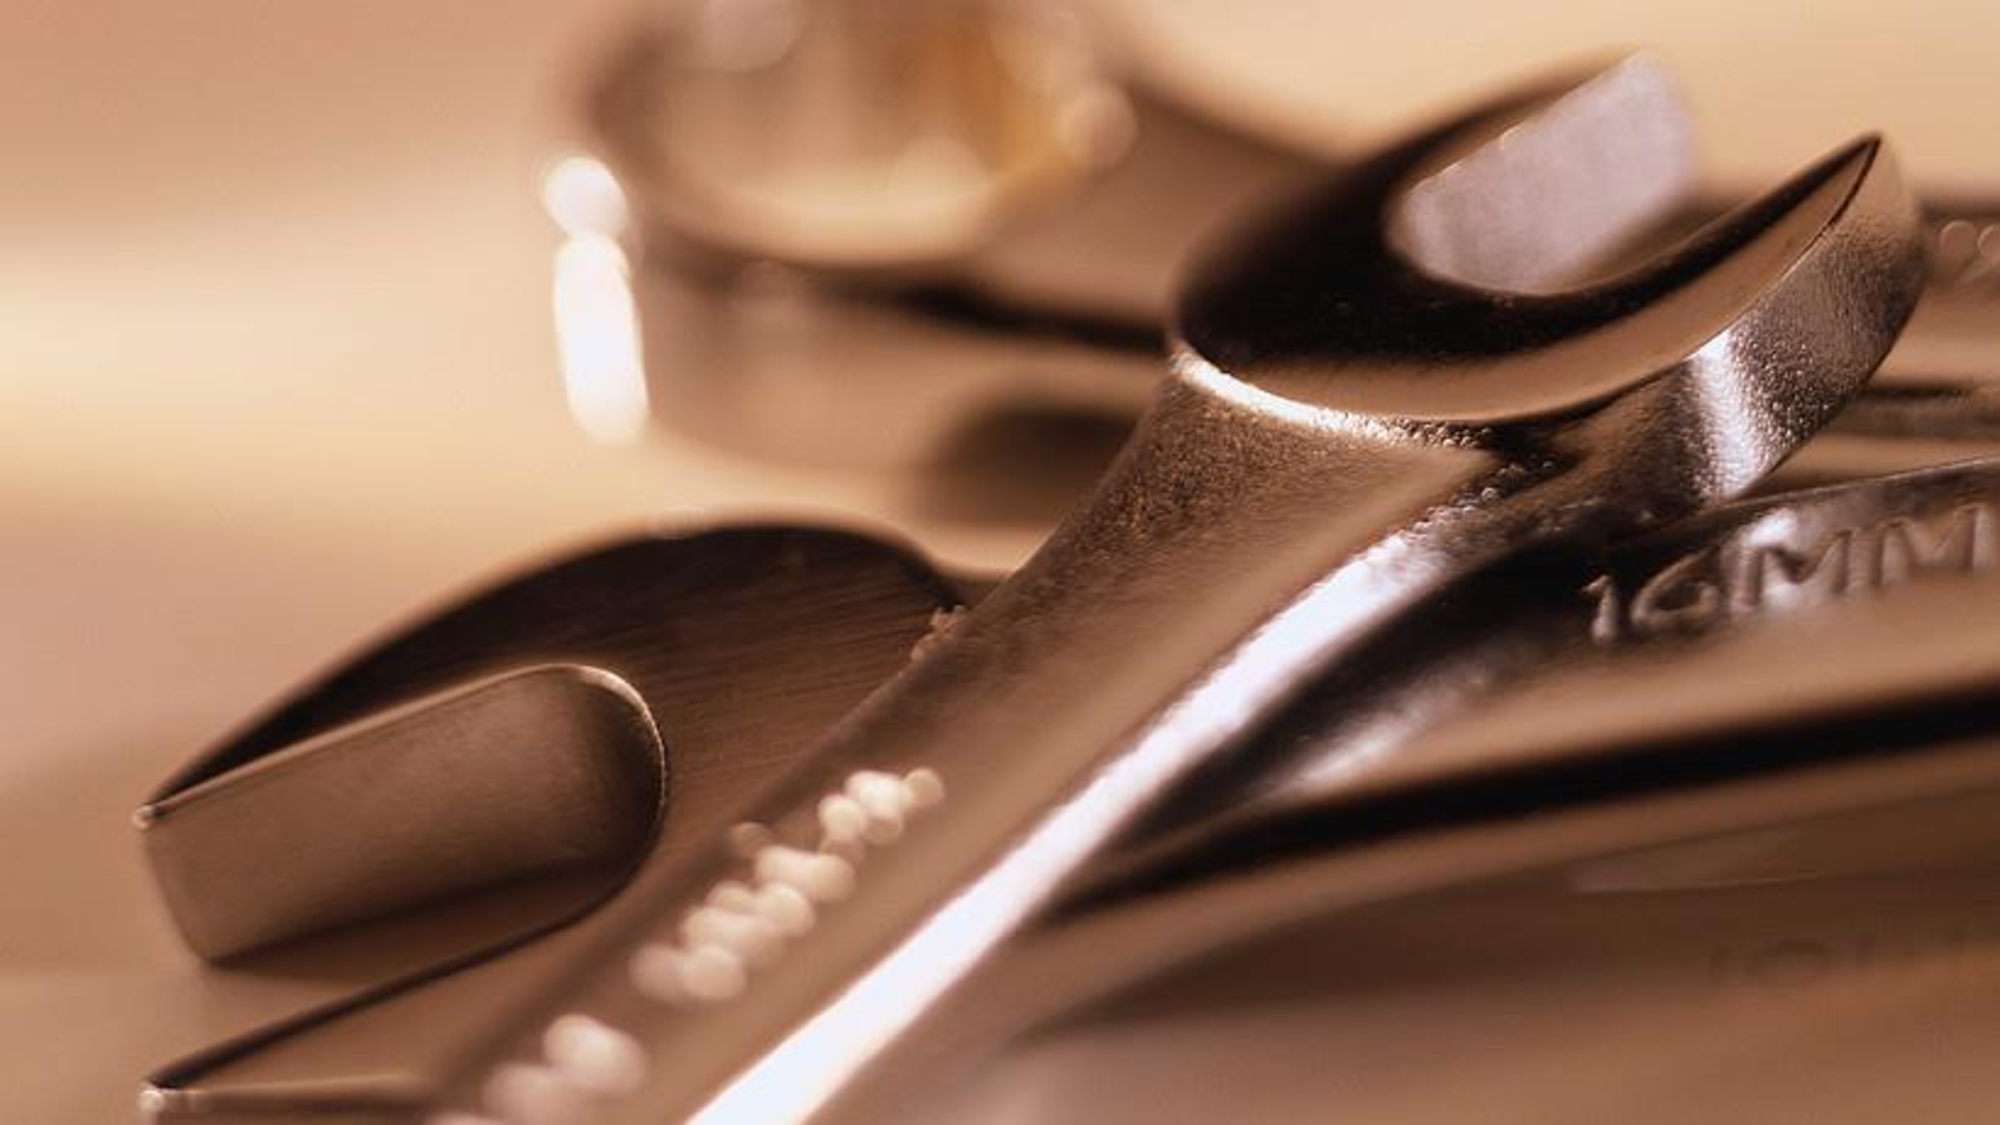
\includegraphics[width=12cm]{Fig/ChangesInManufacturing.pdf}
\caption{製造業におけるニーズとソリューション選択肢の変遷}\label{fig:ChangesInManufacturing}\end{figure}


\subsection{問題の本質の同定}

もともとロボット単体で生産セルを構成するという基本的な考え方は,すでに1980年代の後半に提案されている\cite{Zupancic1988}.当時,人工知能研究もエキスパートシステムと呼ばれる実用化が見られるようになり,バックプロパゲーション則の発見によるニューラルネットワークや,直接法Fuzzy推論則によるFuzzy制御の応用,遺伝的アルゴリズムの応用などが進展しはじめた時代背景とあいまって,生産分野でも,工作機械など熟練者の手に委ねられてきた生産財の知能化研究と実用化が進められてきた.

しかしながら,それらの研究開発成果は,自動化には成功するものの,この手の知的制御システムを
構築するにあたり,熟練作業者モデルを構築するためのシステムの開発,および熟練作業者モデリングの困難さは課題として残ることになった.さらには,1990年代後半から2000年にかけて生産システムの規模が年々大きく複雑化しはじめ,システム構築が属人的技能にとどまっている点も大きな問題となり始めていた\cite{Noda2004}.
2000年代後半になると,産業現場の実務上の問題として,エンジニアリングコストの大きさがシステム構築のボトルネックとなっていることが,はっきりと認識されるようになった.エンジニアリングは,属人的な知識集約作業の典型例であり,リードタイムの長さもコストの一部として計上される.

そこで,著者らの研究グループではこのエンジニアリングコストの削減のため,問題の分析を実施し,本質的な解決策として必要な知能化機能を同定した.これを,第2章で詳報する.

通常,ロボットの知能化というと,外界センサーフードバックにより従来できなかった複雑な動作軌道を実現することに主眼が置かれるが,著者らの研究グループの独創性は,現場のニーズに直接立脚した点にある.
産業用ロボットは生産財である.このため,知能を持った新しいロボットが安全・高速・安定な繰り返し作業を,従来方式となんら変わりなく実現することは大前提である.そのもとで,生産品目切り替えや誤った部品の混入などの大きな外乱に柔軟に対応すること,繰り返し作業への習熟といった自律性を発現する必要がある.
つまり複雑な作業が可能となったとしても動作速度が落ちてしまったり,投資コストが大きくなってしまったりすると,現場では受け入れられない.従来型の生産システムが採用され,極端な場合は作業者を雇い入れるといった解決策が取られることになる.

また,エンジニアリングコストの削減に注目することは,これまでにない視点であり独創性が高い.\cite{robotneeds}%参考文献引用例


\begin{table}[tb]
  \centering
    \caption{値段表}
  \begin{tabular}{|l|c|r||r|} \hline
    メニュー & サイズ & 値段 & カロリー \\ \hline \hline
    牛丼 & 並盛 & 500円 & 600 kcal \\
    牛丼 & 大盛 & 1,000円 & 800 kcal \\
    牛丼 & 特盛 & 1,500円 & 1,000 kcal \\ \hline
  \end{tabular}
\end{table}


\subsection{研究開発のグランドデザインと本論文の主題}

このもとで,知能化技術の要素を開発し,技術プラットフォームとして統合することにした.このことを第3章で詳報する.
そこでは,それぞれの課題の解決のための知能化技術の開発を進めていることを述べる.

研究開発を進めるなかで,人の知能のうち,とりわけ自律性が重要な役割を担っていることがわかったので,製造業向けロボットに自律性を付与する各システムアルゴリズムを開発することにし,これを本論文の主題とした.

まず,人の自律性の最たる特徴の試行錯誤による習熟を,未知の目的関数の最適化問題として定式化して独自の自律システムアルゴリズム「能動型探索アルゴリズム」を提案し,実際のシステムで効果を確認した.また,同種の困難性を持つ問題に対し効果を確認した.これは第4章で詳報する.

次に,自動化システムにおける製品組立作業ではバラ積み状態の部品供給が必ず問題となる.そこで多品種部品のバラ積み供給を実現するシステム設計理論と動作の試行錯誤を実行する「持ち替えグラフアルゴリズム」を提案し,実際の現場で効果を確認した.これは第5章で詳報する.\newpage



\subsection{本論文の構成について}
\noindent
次章以降を,上述した内容に沿って,以下の6つの章で構成する.\\

\noindent
第2章では,自動化システム研究の現状を分析し,課題を明らかにする.\\

\noindent
第3章では,課題を解決するための技術プラットフォーム「自律型セル生産ロボットシステム」の全容について述べる.\\

\noindent
第4章では,課題として重要な自律性の発現について,動作習熟のための自律システムアルゴリズム「能動探索アルゴリズム」について述べる.\\

\noindent
第5章では,おなじく自律性の発現について,バラ積み部品供給のための自律システムアルゴリズム「持ち替えグラフ」について述べる.\\

\noindent
第6章では,実際の製品組立作業を実行するセル生産ロボットシステムを構築して開発技術を検証した結果を報告する.\\

\noindent
第7章で,全体を通じての結論を述べる.\\



\endinput

% for DEBUG % 


% for DEBUG % \setcounter{chapter}{6}
% for DEBUG % 
% !TEX root = thesis.tex
% !TEX encoding = Shift_JIS
% !TEX spellcheck = none


\section{序論}
\subsection{はじめに}

本論文の主題は,第4章と第5章に示す自律システムアルゴリズムである.
同アルゴリズムの研究開発に辿り着くまでには,各時代の要請の変遷とそれを解決するための研究開発の経緯があった.
そこで,なぜ3章以降の開発が必要になったかを明確に定義づけるため,
解説論文的な記述にはなるが,本章と第2章でこれらを示すことにする.

第3章ではそれらを踏まえて開始した,自律型セル生産ロボットシステム技術プラットフォームの
開発プロジェクトの概要について述べる.これはオープンイノベーションを活用した数十人規模の
一大プロジェクトであった.

第4章および第5章で,同プラットフォームに対する要求のなかで最も困難性の高い課題を解決するための
自律システムアルゴリズムについて報告する.




\subsection{背景と動機}

生産人口の減少は,まず日本が,その後,世界が必ず直面する構造問題である.これに対し,あらゆる分野に自動化を万遍なく普及させることが,安全安心で豊かな未来を維持発展させる方法の一つとなる.

製造業分野に目を向けると,動力を利用するようなった産業革命以来,生産を自動化して安価で高品質な製品を大量にライン生産することで,豊かな生活の実現に貢献してきた.
ライン生産方式というソリューションは,設備投資コスト・運用コストを長い期間をかけて回収することが前提であり,つまり概してそれらのコストは大きくなるデメリットがあるものの,一度構築して安定して運用できるようになれば,高速で安定した生産の自動化を維持することにより,同じ品質の製品を大量に製造することができることがメリットとなる.ライン生産方式に投入されるロボットは,この目的のためにその機能を最適設計され,製造されている.そのようなロボットの行動計画は,ライン構築技術者がライン構築時に知恵を絞って設計し,生産活動開始後は,ロボットはあらかじめ定められた単純な位置決め動作を高速に繰り返すことのみに特化していた.これは,動物が条件反射で運動していることに相当する.1990年代にはいると,二次元ビジョンセンサが普及しはじめ,多少の位置ずれをロボット自ら修正する意味での知能化が実用化したが,やはり単純な位置決め動作を高速に繰り返すことに主眼が置かれていて生産ラインの一部への導入にとどまっていた.

2000年代に入ると市場ニーズが多様化しはじめ,短期間のうちに生産機種を切り替える必要が生じた.
このような状況の変化に低コストで柔軟に実施できる人セル生産方式と呼ばれるソリューションが新たな選択肢として注目され,同方式をフル活用したEMS(
\underline{E}lectronics
\underline{M}anufacturing
\underline{S}ervice)事業者も躍進した.
しかし,セル生産方式の生産能力はライン方式に比して低位である.さらには作業者の熟練度に依存する品質のばらつきが直近の課題として取り沙汰されるようになり,これらを解決するために労働者の選抜制をとるなどの方法が取られた.さらには景気の変動に応じて雇用を増減することなどもあわせて,これらの非人道な対応が社会問題となった.また,このような人手をあてにした方式は中長期的には生産人口減少の影響と無縁ではない.

やがて2000年代後半になると,冒頭で述べた生産人口減少問題がようやく人口に膾炙するようになり,
実際に統計的にも日本の人口が減少しはじめ,少子高齢化,生産人口の減少が現実のものとして議論されるようになった.同時に新興国の工業化と市場化の進展により国際競争が激化し,半導体製品・電気電子製品の設計製造技術の革新,景気変動・為替レートの変容・市場ニーズの激変に対応するための市場オフショア生産と地産地消と生産拠点国内回帰の選択の混乱,および市場のグローバル化といった複雑な事象が急速に同時進行したことで,次世代のものつくりの方式が求められ始めていたのが,この2000年代後半の展開であった.

著者らの研究グループでは複雑な状況に対応するためのソリューションの選択肢を増やすため,2006年に新規の研究プロジェクトをスタートさせ,ライン方式,人セル方式,それぞれのメリットを集めたセル生産ロボット方式の実用化を目指すことにした.
ライン生産方式は上述のごとく品種の生産期間は長いことを前提とし少品種大量生産のために最適化され,生産される品質も安定している.ライン生産のなかで産業ロボットは,ワークや治具をピック・アンド・プレースする単純作業に投入されていた.一方,人セル生産方式は生産品種の切り替えが数か月未満で行われることを前提とし,生産速度よりも機種切り替えコストを重視した最適化の結果となっていた.生産速度はラインに比して低いがセルを並列化することで補うという考え方であった.品質は人に依存してばらつきが大きくなっていた.

これに対し,本研究で提案するセル生産ロボット方式では,品種切り替えは迅速,生産速度はそこそこだが品質は安定しているという良いところ取りを目指し,生産速度の増減は,セルの並列数を変化させることで対応しようという概念となる.
ここまで述べてきたことを概念的に図\ref{fig:ChangesInManufacturing}にまとめる.

\begin{figure}[b]\centering 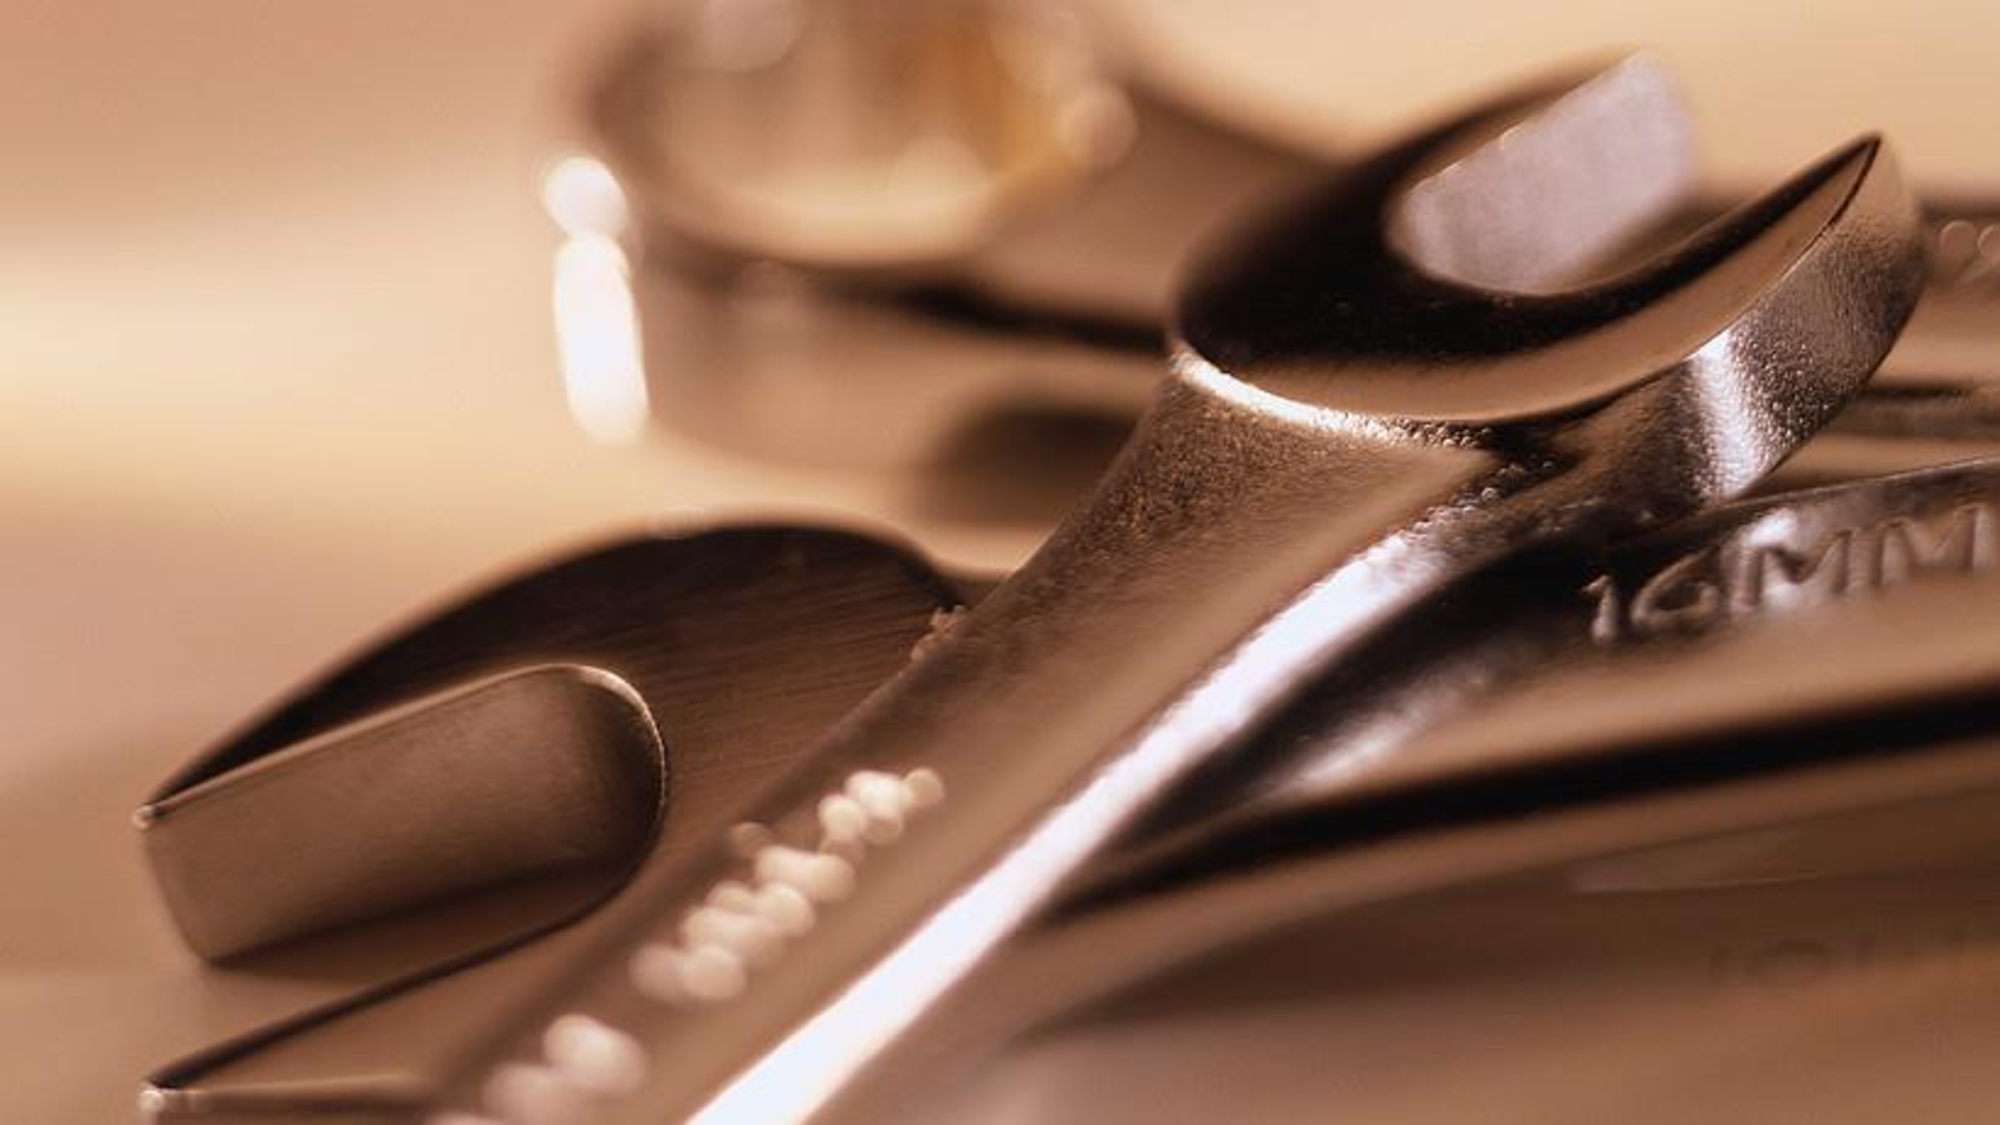
\includegraphics[width=12cm]{Fig/ChangesInManufacturing.pdf}
\caption{製造業におけるニーズとソリューション選択肢の変遷}\label{fig:ChangesInManufacturing}\end{figure}


\subsection{問題の本質の同定}

もともとロボット単体で生産セルを構成するという基本的な考え方は,すでに1980年代の後半に提案されている\cite{Zupancic1988}.当時,人工知能研究もエキスパートシステムと呼ばれる実用化が見られるようになり,バックプロパゲーション則の発見によるニューラルネットワークや,直接法Fuzzy推論則によるFuzzy制御の応用,遺伝的アルゴリズムの応用などが進展しはじめた時代背景とあいまって,生産分野でも,工作機械など熟練者の手に委ねられてきた生産財の知能化研究と実用化が進められてきた.

しかしながら,それらの研究開発成果は,自動化には成功するものの,この手の知的制御システムを
構築するにあたり,熟練作業者モデルを構築するためのシステムの開発,および熟練作業者モデリングの困難さは課題として残ることになった.さらには,1990年代後半から2000年にかけて生産システムの規模が年々大きく複雑化しはじめ,システム構築が属人的技能にとどまっている点も大きな問題となり始めていた\cite{Noda2004}.
2000年代後半になると,産業現場の実務上の問題として,エンジニアリングコストの大きさがシステム構築のボトルネックとなっていることが,はっきりと認識されるようになった.エンジニアリングは,属人的な知識集約作業の典型例であり,リードタイムの長さもコストの一部として計上される.

そこで,著者らの研究グループではこのエンジニアリングコストの削減のため,問題の分析を実施し,本質的な解決策として必要な知能化機能を同定した.これを,第2章で詳報する.

通常,ロボットの知能化というと,外界センサーフードバックにより従来できなかった複雑な動作軌道を実現することに主眼が置かれるが,著者らの研究グループの独創性は,現場のニーズに直接立脚した点にある.
産業用ロボットは生産財である.このため,知能を持った新しいロボットが安全・高速・安定な繰り返し作業を,従来方式となんら変わりなく実現することは大前提である.そのもとで,生産品目切り替えや誤った部品の混入などの大きな外乱に柔軟に対応すること,繰り返し作業への習熟といった自律性を発現する必要がある.
つまり複雑な作業が可能となったとしても動作速度が落ちてしまったり,投資コストが大きくなってしまったりすると,現場では受け入れられない.従来型の生産システムが採用され,極端な場合は作業者を雇い入れるといった解決策が取られることになる.

また,エンジニアリングコストの削減に注目することは,これまでにない視点であり独創性が高い.\cite{robotneeds}%参考文献引用例


\begin{table}[tb]
  \centering
    \caption{値段表}
  \begin{tabular}{|l|c|r||r|} \hline
    メニュー & サイズ & 値段 & カロリー \\ \hline \hline
    牛丼 & 並盛 & 500円 & 600 kcal \\
    牛丼 & 大盛 & 1,000円 & 800 kcal \\
    牛丼 & 特盛 & 1,500円 & 1,000 kcal \\ \hline
  \end{tabular}
\end{table}


\subsection{研究開発のグランドデザインと本論文の主題}

このもとで,知能化技術の要素を開発し,技術プラットフォームとして統合することにした.このことを第3章で詳報する.
そこでは,それぞれの課題の解決のための知能化技術の開発を進めていることを述べる.

研究開発を進めるなかで,人の知能のうち,とりわけ自律性が重要な役割を担っていることがわかったので,製造業向けロボットに自律性を付与する各システムアルゴリズムを開発することにし,これを本論文の主題とした.

まず,人の自律性の最たる特徴の試行錯誤による習熟を,未知の目的関数の最適化問題として定式化して独自の自律システムアルゴリズム「能動型探索アルゴリズム」を提案し,実際のシステムで効果を確認した.また,同種の困難性を持つ問題に対し効果を確認した.これは第4章で詳報する.

次に,自動化システムにおける製品組立作業ではバラ積み状態の部品供給が必ず問題となる.そこで多品種部品のバラ積み供給を実現するシステム設計理論と動作の試行錯誤を実行する「持ち替えグラフアルゴリズム」を提案し,実際の現場で効果を確認した.これは第5章で詳報する.\newpage



\subsection{本論文の構成について}
\noindent
次章以降を,上述した内容に沿って,以下の6つの章で構成する.\\

\noindent
第2章では,自動化システム研究の現状を分析し,課題を明らかにする.\\

\noindent
第3章では,課題を解決するための技術プラットフォーム「自律型セル生産ロボットシステム」の全容について述べる.\\

\noindent
第4章では,課題として重要な自律性の発現について,動作習熟のための自律システムアルゴリズム「能動探索アルゴリズム」について述べる.\\

\noindent
第5章では,おなじく自律性の発現について,バラ積み部品供給のための自律システムアルゴリズム「持ち替えグラフ」について述べる.\\

\noindent
第6章では,実際の製品組立作業を実行するセル生産ロボットシステムを構築して開発技術を検証した結果を報告する.\\

\noindent
第7章で,全体を通じての結論を述べる.\\



\endinput

% for DEBUG % 


% for DEBUG % 
\newpage

%参考文献
\small
\bibliographystyle{jrsj}
\bibliography{Reference}
\normalsize
%% !TEX root = thesis.tex
% !TEX encoding = Shift_JIS
% !TEX spellcheck = none
% 「Reference.bib」を使う場合はこのファイルは使用しない
%
\begin{thebibliography}{99}
\addcontentsline{toc}{section}{参考文献}
\bibitem{Babu} S.S.Babu et al.: ``Empirical model of effects of pressure and temperature on electrical contact resistance of metals,'' Science and Technology of Welding and Joining. vol. 6, no. 12, pp. 126-132, 2001. 
\bibitem{niho} 二保 知也, ほか: ``微視接触電気抵抗解析に基づく抵抗スポット溶接のマルチスケール連成シミュレーション'', 第28回計算力学講演会文集, no. 15-19, 2015. 
\bibitem{Holo} R. Holm: ``Electric Contacts,'' Springer-Verlag, 1958. 
\bibitem{Greenwood} J.A.Greenwood: ``Constriction resistance and the real area of contact,'' British Journal of Applied Physics, vol. 17, no. 3, pp. 1621-1632, 1966. 
\bibitem{OpenCV} Gary Bradski, Adrian Kaehler: ``詳細OpenCV コンピュータビジョンライブラリを使った画像処理・認識'', 株式会社オーム社, 2012, pp. 195-223. 
\bibitem{iroha} 一色 実, 三村 耕司, 鈴木 茂: ``高純度鉄の精製と表面酸化挙動'', 真空, 45, 5, 2002, pp. 395-401. 
\bibitem{samsof} 津田 惟雄, ほか: ``物理科学選書 電気伝導性酸化物(改訂版)'', 裳華房, 1993, p. 26. 
\bibitem{honma} 本間 禎一: ``酸化皮膜の機械的性質と金属の酸化'', 防食技術, 25, 4, 1976, pp. 251-265. 
\bibitem{oya} 倉前 宏行, ほか: ``マルチスケール抵抗スポット溶接解析のための微視有限要素モデルの検討'', 第30回計算力学講演会論文集, 2017. 
\end{thebibliography}

\section*{本研究に関する発表リスト}
\addcontentsline{toc}{section}{本研究に関する発表}
\begin{enumerate}
\renewcommand{\labelenumi}{[\arabic{enumi}]}
\item
倉前宏行, 二保知也, 荒牧弘親, 大矢健吾, 堀江知義:マルチスケール抵抗スポット溶接解析のための微視有限要素モデルの検討, 日本機械学会 第30回計算力学講演会, 近畿大学東大阪キャンパス(大阪府東大阪市), 2017年9月16日

\item
倉前宏行, 大矢健吾:抵抗スポット溶接のマルチスケール・マルチフィジックス有限要素シミュレーション, 若手研究室見本市「イノベーションOIT 2017」, 大阪工業大学大宮キャンパス, 2017年10月26日
\end{enumerate}




\endinput
%参考文献
% for DEBUG % 


% for DEBUG % 
% !TEX root = thesis.tex
% !TEX encoding = Shift_JIS
% !TEX spellcheck = none


\section*{謝辞}
%\addcontentsline{toc}{chapter}{謝辞}

本研究を論文にまとめるにあたり,非常に多くの方々のご指導・ご協力を賜りましたことに心より感謝申し上げます.

主指導教員 大学 小笠原司教授,副指導教員 同 杉本謙二教授,高松淳准教授,丁明助教から,
数多くの丁寧かつ適切なご指導をいただきました.

同学ロボティクス研究室のスタッフ・OB・学生の皆様,同学の皆様には研究会・授業・公聴会ほか,
様々な議論の機会を通じて重要な示唆をいただき,また学生生活に関するお力添えをいただきました.


本研究の一部は``METI・NEDO次世代ロボット知能化技術開発プロジェクト'',``NEDO戦略的先端ロボット要素技術開発プロジェクト''の委託を受けて実施しました.


\endinput
%謝辞
%\newpage
%\thispagestyle{empty}



\end{document}


